% Manuscript prepared for submission to Computers in Biology and Medicine (Elsevier)
% Generic article class used for review submission
\documentclass[11pt,a4paper]{article}

\usepackage{lmodern}
\usepackage{float}
\usepackage{amsmath,amssymb}
\usepackage[mathlines]{lineno}
\usepackage{graphicx}
\usepackage{booktabs}
\usepackage{array}
\usepackage{multirow}
\usepackage[colorlinks=true,linkcolor=blue,citecolor=blue,urlcolor=blue]{hyperref}
\usepackage{caption}
\usepackage{subcaption}
\usepackage[numbers,sort&compress,square]{natbib}
\usepackage[top=1.00in,bottom=1.00in,left=1.25in,right=1.25in]{geometry}
\usepackage{microtype}
\usepackage{orcidlink}
\usepackage{marvosym}
\usepackage{etoolbox}
\AtBeginEnvironment{tabular}{\footnotesize}
\usepackage{placeins}
\usepackage{titlesec}
\usepackage{titling}
\setlength{\droptitle}{-3em}
\usepackage{setspace}
\doublespacing

% Section / subsection heading spacing
\titlespacing*{\section}{0pt}{8pt plus 2pt minus 1pt}{4pt plus 1pt}
\titlespacing*{\subsection}{0pt}{6pt plus 2pt minus 1pt}{3pt plus 1pt}
\titlespacing*{\subsubsection}{0pt}{4pt}{2pt}

% Float and caption spacing
\setlength{\textfloatsep}{5pt plus 1pt minus 1pt}
\setlength{\floatsep}{4pt plus 1pt minus 1pt}
\setlength{\intextsep}{4pt plus 1pt minus 1pt}
\setlength{\abovecaptionskip}{2pt}
\setlength{\belowcaptionskip}{1pt}

% Equation display spacing
\setlength{\abovedisplayskip}{5pt plus 2pt minus 2pt}
\setlength{\belowdisplayskip}{5pt plus 2pt minus 2pt}
\setlength{\abovedisplayshortskip}{3pt plus 1pt}
\setlength{\belowdisplayshortskip}{3pt plus 1pt}

% Caption font size
\captionsetup{font=footnotesize,labelfont=bf,labelsep=space}
\renewcommand{\figurename}{Fig.}

% Bibliography entry spacing
\setlength{\bibsep}{2pt}

\title{\textbf{Toward Risk-Aware Clinical Decision Support in Gastrointestinal Endoscopy:\\
A Tunable Asymmetric Loss with Uncertainty-Guided Referral}}

\author{%
  Azizur Rahman$^{1}$\orcidlink{0009-0007-6945-6953} \and
  Nakib Uddin Ahmed$^{2}$\orcidlink{0009-0006-6515-5750} \and
  Kadirur Rahman Chowdhury$^{3}$ \and
  Mehjabin Ferdous$^{4}$ \and
  J.S.\ Jannatun Nayema$^{5}$ \and
  Md.\ Shahadat Hossain$^{6}$ \and
  Akhlak Uz Zaman$^{7}$\orcidlink{0000-0001-6327-6942}
}

\date{}

\begin{document}

\maketitle
\vspace{2pt}

\begin{singlespace}
\begin{abstract}
This study presents a deep learning framework for four-class gastrointestinal
(GI) endoscopy risk stratification beyond conventional binary lesion
detection. Images from the HyperKvasir dataset were categorized into four
clinically motivated risk groups: Normal, Inflammatory, Pre-malignant, and
High-Risk, informed by recommendations from the American College of
Gastroenterology and European Society of Gastrointestinal Endoscopy. We
introduce an Asymmetric Endoscopy Loss (AEL) function that enables tunable
class weighting, allowing greater emphasis on High-Risk cases while
balancing overall predictive performance with safety-oriented sensitivity.
Three lightweight architectures (DenseNet-121, EfficientNet-B0, and
DeiT-Tiny) were evaluated using AEL, with Monte Carlo Dropout for
uncertainty estimation and a referral strategy that escalates Pre-malignant
and High-Risk predictions for further review regardless of model confidence.
GradCAM was used to provide visual interpretability. DenseNet-121 achieved a
macro F1-score of 0.8419 and an AUC of 0.9730. No ground-truth High-Risk
images were predicted as either of the two lower-risk tiers on the internal
test set, and 43.1\,\% of images were eligible for simulated automatic
clearance under the predefined referral rule.
Five-fold cross-validation provided an additional assessment of performance
stability, while McNemar tests quantified paired differences between
architectures. These findings support further investigation of
tunable risk-weighted losses, lightweight architectures, and
uncertainty-aware referral strategies for developing interpretable and
safety-oriented GI endoscopy decision-support systems.
\end{abstract}

\noindent\textbf{Keywords:}
Clinical decision support;
Cost-sensitive learning;
Explainable artificial intelligence;
Gastrointestinal endoscopy;
Risk stratification;
Uncertainty quantification
\end{singlespace}

\linenumbers

%% ============================================================================
\section{Introduction}
\label{sec:intro}
%% ============================================================================

Gastrointestinal (GI) cancers, including colorectal, gastric, and esophageal malignancies, represent a substantial global health burden and remain an important cause of cancer-related mortality~\citep{Sung2021}. Early detection of clinically significant abnormalities during endoscopic examination is essential for improving patient outcomes; however, subtle mucosal abnormalities may be overlooked because of lesion characteristics, inter-endoscopist variability, and operator fatigue during high-volume examinations~\citep{Kaminski2017}. Computer-aided detection (CAD) and computer-aided diagnosis systems have therefore received increasing attention as tools for assisting endoscopists in lesion detection and characterization. Randomized controlled trials have reported improvements in selected endoscopic detection tasks with AI-assisted systems~\citep{Wang2019}, and several AI-based technologies have subsequently progressed toward clinical use. Nevertheless, many existing endoscopic AI systems remain primarily focused on binary detection or classification tasks, such as distinguishing lesion-present from lesion-absent images or normal from abnormal findings~\citep{Ahmad2021}.

A binary classification framework provides limited information for clinical decision-making because endoscopic findings may differ substantially in their associated clinical risk and subsequent management. Current recommendations from organizations such as the American College of Gastroenterology (ACG) and the European Society of Gastrointestinal Endoscopy (ESGE) incorporate differences in lesion characteristics, dysplasia, malignancy risk, and other clinical factors when determining biopsy, surveillance, resection, or additional treatment strategies~\citep{Shaukat2021,Ferlitsch2017}. For example, current ACG guidance addresses surveillance and treatment according to the underlying condition and degree of dysplasia, while ESGE recommendations similarly distinguish among lesions according to their malignant potential and endoscopic characteristics~\citep{Ferlitsch2017}. These recommendations illustrate that clinically relevant endoscopic assessment is inherently more nuanced than a simple binary decision.

The consequences of classification errors are also unlikely to be uniform across risk levels. A false-negative prediction for a clinically significant or high-risk lesion may delay biopsy, surveillance, or therapeutic intervention, whereas an erroneous high-risk prediction for a benign finding may result primarily in additional diagnostic evaluation or follow-up. This asymmetry motivates the development of machine-learning objectives that account not only for class imbalance but also for the relative clinical consequences of different types of misclassification. Conventional cross-entropy and Focal Loss~\citep{Lin2017} primarily optimize predictive performance without explicitly encoding such task-specific differences in error costs.

Previous deep learning studies in GI endoscopy have predominantly investigated lesion detection, polyp detection, or binary classification~\citep{Tajbakhsh2016,Ahmad2021}. Multi-class classification has also been explored for specific lesion types and anatomical settings, including risk assessment of gastric subepithelial lesions~\citep{Ebigbo2019}. However, a unified multi-class framework for risk-oriented analysis across heterogeneous GI endoscopic findings remains comparatively underexplored. In particular, there is limited work investigating whether a risk-oriented, clinically informed asymmetric loss function can be combined with lightweight deep learning architectures, uncertainty estimation, and explainability within a common evaluation framework.

In this study, we formulate GI endoscopic image analysis as a four-class risk stratification problem consisting of Normal, Inflammatory, Pre-malignant, and High-Risk categories. These categories are defined at the study level and are informed by clinically relevant distinctions in endoscopic findings, dysplasia, malignant potential, and management pathways described in existing clinical guidance~\citep{Shaukat2021,Ferlitsch2017}. The objective is not to reproduce any single clinical guideline or replace histopathological diagnosis, but rather to investigate whether risk-oriented categorization can provide a more clinically informative formulation than binary lesion detection.

To address the unequal consequences associated with different classification errors, we introduce a tunable risk-oriented cost-sensitive weighted cross-entropy formulation, the Asymmetric Endoscopy Loss (AEL), that provides a tunable mechanism for encoding the relative importance of errors involving higher-risk categories directly into model optimization. In the proposed formulation, misclassification of High-Risk cases receives a fivefold penalty relative to the baseline class weighting, and this penalty can be adjusted to trade off overall predictive accuracy against safety-oriented recall for the highest-risk tier. This design allows the assumed risk hierarchy to be incorporated into training while preserving a standard supervised classification framework. The proposed approach is evaluated using three lightweight architectures (DenseNet-121, EfficientNet-B0, and DeiT-Tiny), each with fewer than eight million parameters, enabling a comparison between convolutional and transformer-based representations under a similar computational constraint.

Beyond predictive performance, uncertainty estimation and model interpretability are incorporated to examine the potential utility of the proposed framework in risk-oriented referral settings. Monte Carlo Dropout~\citep{Gal2016} is employed to estimate predictive uncertainty by retaining dropout during inference. Rather than relying solely on confidence thresholds, we additionally investigate a rule-based referral strategy in which predictions categorized as Pre-malignant or High-Risk are escalated for further review regardless of model confidence. This design reflects the intended use of the system as a decision-support mechanism rather than an autonomous diagnostic tool. Gradient-weighted Class Activation Mapping (GradCAM) is subsequently used to visualize image regions contributing to model predictions and to facilitate qualitative examination of model behavior.

The models are evaluated on the HyperKvasir dataset under a common experimental protocol and subsequently assessed for zero-shot generalization on the independent Kvasir-v2 dataset. Five-fold cross-validation is used to examine the stability of model performance, while McNemar's test is employed for statistical comparison of paired classification outcomes. An ablation analysis further evaluates the contribution of AEL relative to conventional cross-entropy and Focal Loss. The resulting framework therefore integrates asymmetric cost-sensitive learning, lightweight architectures, uncertainty estimation, and visual explanation within a unified evaluation setting.

The main contributions of this work are the following:

\begin{itemize}
\item we formulated GI endoscopic image classification as a four-class risk stratification problem comprising Normal, Inflammatory, Pre-malignant, and High-Risk categories, providing a more granular representation than binary lesion classification;
\item we introduced the Asymmetric Endoscopy Loss (AEL), a risk-oriented, clinically informed and tunable weighted loss function that assigns increased penalty to misclassification of higher-risk findings, with a fivefold weighting for High-Risk errors, providing a controllable mechanism for trading off overall accuracy against safety-oriented recall rather than a guaranteed performance improvement;
\item we systematically evaluated DenseNet-121, EfficientNet-B0, and DeiT-Tiny under a common sub-8-million-parameter constraint, enabling comparison of convolutional and transformer-based architectures;
\item we combined Monte Carlo Dropout with a risk-based escalation protocol to investigate whether uncertainty estimation and predetermined risk thresholds can support referral-oriented decision-making;
\item we employed GradCAM for visual interpretation, conducted five-fold cross-validation and statistical testing, and evaluated zero-shot generalization on the independent Kvasir-v2 dataset.
\end{itemize}

Overall, this study presents a computational investigation of risk-oriented GI endoscopic image classification rather than a clinically validated diagnostic system. The framework is intended to examine the feasibility of incorporating asymmetric error costs, lightweight deep learning, uncertainty estimation, and visual explanation into AI-assisted endoscopic risk stratification. Further prospective validation, expert assessment, and clinical studies will be required before such a system can be considered for clinical deployment.

%% ============================================================================
\section{Related Work}
\label{sec:relwork}
%% ============================================================================

\subsection{Deep Learning for GI Endoscopy Classification}
Early applications of deep learning to gastrointestinal endoscopy primarily
focused on automated detection and classification of specific lesions,
particularly colorectal polyps. Tajbakhsh et~al.~\citep{Tajbakhsh2016}
demonstrated the application of convolutional neural networks (CNNs) for
automated polyp detection in colonoscopy images and video. Subsequent
randomized controlled trials reported improvements in selected adenoma
detection outcomes when computer-aided detection systems were used during
colonoscopy~\citep{Wang2019}. These studies established the potential of deep
learning as an assistive technology for endoscopic examination, while also
highlighting the importance of evaluating such systems under clinically
relevant conditions.

Beyond binary lesion detection, Pogorelov et~al.~\citep{Pogorelov2017}
investigated multi-class classification using the eight-class Kvasir-v1
dataset. The subsequent HyperKvasir dataset~\citep{Borgli2020} expanded the
diversity of GI findings, providing 23 annotated classes across 10,662
labelled images. These datasets have facilitated the development and
benchmarking of deep learning methods for GI image classification across
different finding categories. However, the majority of existing approaches
formulate the task around anatomical findings or individual lesion types
rather than explicitly organizing findings according to their potential
clinical risk.

Systematic reviews of computer-aided colonoscopy have identified several
challenges affecting the translation of AI systems into clinical practice,
including class imbalance, domain shift, variability in image acquisition,
and limited integration with clinical workflows~\citep{Ahmad2021}. These
challenges are particularly relevant when models are evaluated outside the
dataset on which they were trained. Accordingly, evaluation across independent
datasets can provide additional information about model generalization and
robustness.

A substantial body of recent GI endoscopy research has also focused on polyp
segmentation. The Kvasir-SEG dataset~\citep{Jha2020} has become an established
benchmark for this task, and numerous segmentation architectures have
subsequently been evaluated on the dataset. Although segmentation provides
detailed localization of lesions, it does not directly address the broader
problem of assigning heterogeneous GI findings to clinically meaningful risk
categories. Ebigbo et~al.~\citep{Ebigbo2019}, for example, investigated
malignancy risk classification for gastric subepithelial lesions,
demonstrating the potential of AI-based approaches for risk-oriented
endoscopic assessment. Such approaches, however, generally focus on specific
lesion types or anatomical sites.

In contrast, the present study investigates a unified four-class risk
stratification framework spanning heterogeneous GI endoscopic findings.
Rather than treating all classification errors as equivalent, the proposed
framework considers differences in the potential clinical implications of
errors across risk categories and evaluates whether this distinction can be
incorporated into model training and referral strategies.

\subsection{Asymmetric and Cost-Sensitive Losses in Medical Imaging}
Conventional cross-entropy loss treats individual classification errors
according to the specified class weights but does not inherently represent an
ordered relationship between clinical severity levels. Focal Loss~\citep{Lin2017}
modifies the contribution of training examples according to prediction
difficulty and has been widely used to address class imbalance in computer
vision and medical image classification. However, prediction difficulty and
clinical severity represent different concepts; consequently, Focal Loss does
not explicitly encode the relative clinical consequences of confusing one risk
category with another.

Cost-sensitive learning provides an alternative approach by assigning
different penalties to different classes or error types. Class-weighted
cross-entropy and related cost-sensitive objectives have been investigated in
medical imaging applications including diabetic retinopathy grading,
skin-lesion classification, and histopathological classification. These
methods are motivated by the observation that errors involving severe disease
categories may have greater clinical significance than errors involving
lower-risk categories.

Building on this principle, we introduce the Asymmetric Endoscopy Loss (AEL)
for four-class GI risk stratification. AEL assigns greater training weight to
errors involving higher-risk categories, with a fivefold penalty applied to
High-Risk misclassification in the proposed formulation. The objective is to
incorporate the predefined risk hierarchy into model optimization rather than
relying exclusively on post-hoc decision thresholds. This formulation is
intended as a computational representation of task-specific error costs and
should not be interpreted as a direct quantitative measure of patient
mortality or clinical outcome.

\subsection{Compact Vision Transformers and CNN-Transformer Architectures}
Transformer-based architectures have increasingly been investigated for
medical image analysis because self-attention can model long-range
relationships between image regions. However, the computational and data
requirements of conventional Vision Transformers can limit their applicability
to relatively small medical imaging datasets. DeiT~\citep{Touvron2021}
demonstrated that knowledge distillation can substantially improve the data
efficiency of Vision Transformers, enabling compact models such as DeiT-Tiny
to operate with considerably fewer parameters than large ViT
architectures~\citep{Dosovitskiy2021}.

CNNs and Transformer-based models provide complementary inductive biases for
visual representation. CNNs emphasize local spatial patterns through
convolutional operations, whereas self-attention enables interactions among
image patches over a broader spatial context. CNN-Transformer hybrid
architectures have consequently been explored extensively in medical image
analysis, particularly for segmentation and classification tasks.

The HyperKvasir dataset presents a challenging setting for this comparison
because the labelled images represent heterogeneous GI findings while
remaining substantially smaller than datasets commonly used to train
large-scale vision models. In this study, DenseNet-121, EfficientNet-B0, and
DeiT-Tiny are evaluated under a common sub-eight-million-parameter constraint.
This design enables comparison across convolutional and Transformer-based
architectures while reducing differences attributable solely to model scale.
The comparison therefore focuses on the effects of architectural
representation and inductive bias within a lightweight computational setting.

\subsection{Uncertainty Quantification in Clinical Decision Support}
Predictive uncertainty is an important consideration when machine-learning
models are used in clinical decision-support settings. A highly confident
incorrect prediction may be more difficult to identify than an uncertain
prediction, particularly when the system is used to assist rather than replace
expert assessment. Monte Carlo Dropout provides an efficient approach for
estimating model uncertainty by retaining dropout during inference and
obtaining multiple stochastic predictions~\citep{Gal2016}. The resulting
prediction distribution can be used to characterize uncertainty without
requiring the computational cost of training a large ensemble of independently
parameterized models.

In medical image analysis, uncertainty estimation has been investigated as a
mechanism for identifying cases that may require additional expert review.
Within GI endoscopy, confidence-based referral strategies have been explored
for lesion assessment, including approaches that escalate predictions falling
below predefined confidence thresholds~\citep{Ebigbo2019}. Such strategies
can potentially reduce reliance on fully automated decisions in ambiguous
cases.

The present study investigates a complementary risk-based referral strategy.
Rather than using model confidence as the sole criterion for escalation,
predictions assigned to the Pre-malignant and High-Risk categories are
automatically referred for further review. This rule is designed to prioritize
sensitivity to higher-risk categories independently of the model's estimated
confidence. Importantly, this should be interpreted as a
predefined referral rule within the experimental framework, rather
than as a clinical safety guarantee. Its effectiveness is evaluated
empirically using the internal test set and should not be generalized to
clinical practice without prospective validation.

%% ============================================================================
\section{Materials and Methods}
\label{sec:methods}
%% ============================================================================

\begin{figure}[H]
  \centering
  \includegraphics[width=\textwidth]{framework.png}
  \caption{Overview of the proposed GI endoscopy risk stratification
    framework. Raw endoscopic images undergo contrast enhancement using
    Contrast Limited Adaptive Histogram Equalization (CLAHE) before being
    processed by three lightweight deep learning architectures, each
    containing fewer than 8 million parameters. The models are trained
    using the proposed Asymmetric Endoscopy Loss (AEL) and produce
    predictions for four risk categories: Normal, Inflammatory,
    Pre-malignant, and High-Risk. Monte Carlo Dropout is subsequently used
    to estimate predictive uncertainty and support the predefined referral
    strategy, while GradCAM heatmaps are generated to visualize image
    regions associated with model predictions}
  \label{fig:framework}
\end{figure}

Figure~\ref{fig:framework} illustrates the overall workflow of the
proposed framework, beginning with raw GI endoscopic images and
proceeding through image preprocessing, model inference, uncertainty
estimation, risk-based referral, and visual interpretation. Following
CLAHE preprocessing, the images are independently evaluated using three
lightweight architectures: DenseNet-121, EfficientNet-B0, and DeiT-Tiny.
Each architecture is trained under the proposed AEL objective to account
for the predefined differences in classification costs across risk
categories. The resulting predictions are evaluated using Monte Carlo
Dropout to estimate predictive uncertainty. A predefined referral
protocol is then applied, with Pre-malignant and High-Risk predictions
designated for further review regardless of the estimated model
confidence. Finally, GradCAM is used to generate class-specific
activation maps that provide a visual representation of the image regions
contributing to the model predictions.

\subsection{Datasets}
\label{sec:datasets}

We used HyperKvasir~\citep{Borgli2020} as the primary training and evaluation
dataset. HyperKvasir is a large publicly available annotated GI endoscopy
dataset comprising 110,079 images from upper and lower GI tract examinations
collected at Baerum Hospital, Norway. The labeled image subset contains 10,662
images across 23 finding classes, organized in a nested directory structure
according to GI tract region, anatomical category, and finding class. Images
are provided as JPEG files with variable resolutions and were resized to
$224\times224$ pixels prior to training.

For external validation, we used Kvasir-v2~\citep{Pogorelov2017b}, an
independent dataset containing 8,000 images across eight GI finding classes
collected from a different patient population and imaging equipment. Kvasir-v2
was used exclusively for zero-shot evaluation; no Kvasir-v2 images were used
during training, validation, or hyperparameter selection. This design evaluates
the ability of models trained on HyperKvasir to generalize to a clinically and
technically distinct cohort. The eight Kvasir-v2 classes were mapped to the
same four-tier risk schema used for HyperKvasir, following the ACG/ESGE-based
criteria described in the study. The complete class mapping is provided
alongside the zero-shot evaluation results in Section~\ref{sec:results}.

For HyperKvasir, the labeled images were mapped to four risk tiers: Normal,
Inflammatory, Pre-malignant, and High-Risk. Two non-pathological classes,
\texttt{bbps-0-1} and \texttt{impacted-stool}, were excluded from the analysis
because they do not correspond to the target risk-stratification schema. After
class mapping and exclusion, the resulting usable HyperKvasir subset contained
7,633 images: 3,000 Normal, 645 Inflammatory, 1,836 Pre-malignant, and 2,152
High-Risk images.

The usable HyperKvasir subset was divided at the image level using stratified
sampling into training (70\%), validation (15\%), and test (15\%) sets. A fixed
random seed (SEED\,$=$\,42) was used to ensure reproducibility. Because the
four risk tiers were substantially imbalanced, particularly the Inflammatory
class, the training set was balanced using \texttt{WeightedRandomSampler} with
sampling weights inversely proportional to class frequencies. This ensured
approximately equal expected representation of the four classes during training.

\begin{figure}[H]
  \centering
  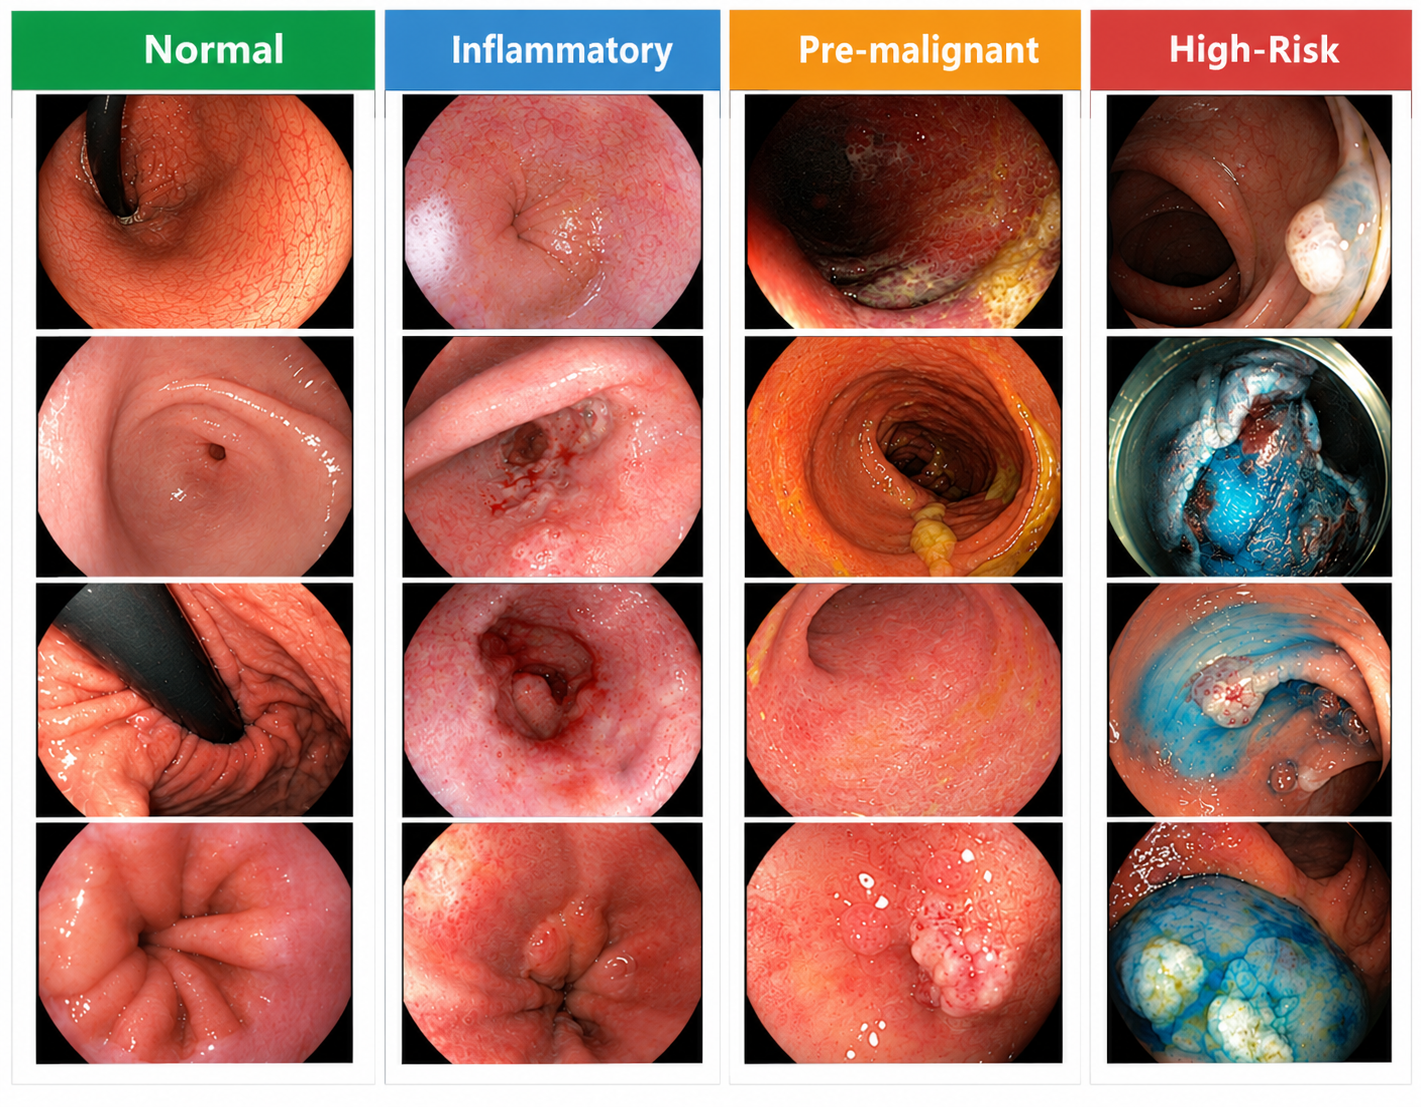
\includegraphics[width=0.7\textwidth]{samples_hyperkvasir.png}
  \caption{Representative HyperKvasir endoscopy images per risk tier.
    Each column corresponds to one risk class (Normal, Inflammatory,
    Pre-malignant, High-Risk)}
  \label{fig:samples}
\end{figure}

Figure~\ref{fig:samples} presents representative endoscopy images from each
risk tier in HyperKvasir, illustrating the visual diversity within each
risk category on the primary training and evaluation dataset.

The Inflammatory tier was the smallest class in HyperKvasir, with 645 images,
motivating the use of \texttt{WeightedRandomSampler} during training and macro
F1 as the primary evaluation metric. In contrast, the Kvasir-v2 subset used
for zero-shot evaluation contains 1,000 images per risk tier, resulting in a
balanced external evaluation set.


\subsection{Study-Defined Risk Stratification Schema}
\label{sec:schema}

It is important to state precisely what the four-class schema used in this
study is, and what it is not. The schema is a study-defined risk
stratification categorization informed by ACG/ESGE guidance, not an
established clinical classification system endorsed or defined by these
societies. The ACG and ESGE guidelines describe intervention pathways for
specific, individually diagnosed findings (e.g., specific dysplasia grades,
specific polyp histology); they do not themselves define a single four-tier
labeling scheme spanning the heterogeneous finding categories present in
HyperKvasir. The mapping from HyperKvasir finding labels to the four study
tiers, Normal, Inflammatory, Pre-malignant, and High-Risk, was therefore
constructed at the study level by the authors, using the general
intervention pathways described in ACG and ESGE guidance
documents~\citep{Shaukat2021,Ferlitsch2017} as a reference point, and was
independently cross-checked against the published criteria by co-author
Mehjabin Ferdous (MPH, St.\ Francis College). The complete mapping is
provided in Table~\ref{tab:schema}.

The rationale for specific class assignments is as follows. Findings
representing normal anatomical landmarks and adequately prepared bowel
segments (e.g., \texttt{cecum}, \texttt{pylorus}, \texttt{z-line},
\texttt{bbps-2-3}) were assigned to Normal because they do not
correspond to a pathological finding requiring follow-up beyond routine
screening intervals. Early-grade inflammatory findings (e.g.,
\texttt{esophagitis-a}, \texttt{ulcerative-colitis-grade-0-1},
\texttt{hemorrhoids}) were separated from more advanced inflammatory and
pre-malignant findings and assigned to Inflammatory because ACG/ESGE
guidance generally directs these toward non-urgent medical management rather
than biopsy or intensified surveillance. \texttt{Polyps} and Barrett's-related
findings were assigned to Pre-malignant because colorectal polyps
and Barrett's esophagus are established precursor lesions for which
guidelines recommend tissue sampling and defined surveillance intervals,
reflecting a meaningfully different management pathway from either normal
findings or early inflammatory disease. \texttt{Dyed-lifted-polyps} and
\texttt{dyed-resection-margins} were assigned to High-Risk not
because dye-assisted imaging itself indicates malignancy, but because these
HyperKvasir classes specifically depict images captured during or
immediately after endoscopic mucosal resection, a procedure performed when a
lesion has already been assessed by the endoscopist as warranting removal;
these images therefore represent the intervention stage associated with the
most clinically significant lesions in the dataset. More advanced
inflammatory grades (e.g., \texttt{ulcerative-colitis-grade-2-3},
\texttt{ulcerative-colitis-grade-3}) were likewise assigned to
High-Risk because ACG/ESGE guidance associates high-grade,
extensive inflammatory disease with escalated management and closer
specialist oversight relative to mild or localized disease.

We emphasize that this schema is intended as a research framework for
informatics and decision-support purposes, that is, to investigate whether
a risk-oriented categorization of endoscopic findings can support more
clinically informative model training and referral behavior than binary
lesion detection, rather than as a diagnostic classification system. It
does not substitute for histopathological diagnosis, and individual
assignments (particularly the grouping of heterogeneous findings within the
Pre-malignant and High-Risk tiers) should be understood as simplifications
made for the purposes of this computational study.

Two HyperKvasir classes, \texttt{bbps-0-1} and \texttt{impacted-stool},
were excluded because they represent bowel-preparation quality and a
non-pathological examination state, respectively, rather than disease findings
suitable for risk stratification. After exclusion, 21 HyperKvasir
finding classes remained and were assigned to the four risk categories.

\begin{table}[H]
\centering
\caption{Study-defined four-class risk stratification schema informed by
  ACG/ESGE guideline-based management considerations}
\label{tab:schema}
\begin{tabular}{clp{5.8cm}p{3.8cm}}
\toprule
\textbf{Class} & \textbf{Label} &
\textbf{HyperKvasir Source Classes} &
\textbf{Guideline-Aligned Management Category}\\
\midrule
0 & \textbf{Normal} &
  \raggedright\textit{cecum}, \textit{pylorus}, \textit{z-line},
  \textit{retroflex-stomach}, \textit{retroflex-rectum},
  \textit{ileum}, \textit{bbps-2-3}\arraybackslash &
  Routine surveillance according to applicable screening guidelines\\[2pt]
1 & \textbf{Inflammatory} &
  \raggedright\textit{esophagitis-a},
  \textit{ulcerative-colitis-grade-0-1},
  \textit{ulcerative-colitis-grade-1},
  \textit{hemorrhoids}\arraybackslash &
  Medical management with non-urgent clinical follow-up\\[2pt]
2 & \textbf{Pre-malignant} &
  \raggedright\textit{barretts}, \textit{barretts-short-segment},
  \textit{esophagitis-b-d}, \textit{polyps},
  \textit{ulcerative-colitis-grade-1-2},
  \textit{ulcerative-colitis-grade-2}\arraybackslash &
  Tissue sampling and/or short-interval surveillance\\[2pt]
3 & \textbf{High-Risk} &
  \raggedright\textit{ulcerative-colitis-grade-2-3},
  \textit{ulcerative-colitis-grade-3},
  \textit{dyed-lifted-polyps},
  \textit{dyed-resection-margins}\arraybackslash &
  Urgent specialist evaluation and consideration of intervention\\
\bottomrule
\end{tabular}
\par\smallskip
{\footnotesize\textit{The management categories above are illustrative
risk-stratification categories intended to provide clinical interpretability
rather than treatment recommendations. Actual patient management depends on
physician judgment, individual patient characteristics, diagnostic findings,
and the complete recommendations of the applicable ACG and ESGE guidelines.}}
\end{table}

\subsection{Image Preprocessing and Augmentation}
\label{sec:preproc}

Endoscopic images often exhibit non-uniform illumination, variable image
quality, and limited mucosal contrast. To improve local contrast while
limiting noise amplification, we applied Contrast-Limited Adaptive Histogram
Equalization (CLAHE)~\citep{Reza2004} to the L-channel of each image
after conversion to the CIE L*a*b* color space. CLAHE was configured with a
clip limit of 2.0 and an 8\,$\times$\,8 tile grid. Applying
CLAHE to the luminance channel enhances local mucosal texture and vascular
patterns while preserving the original chromatic information.

For the training set, images were first resized to 256\,$\times$\,256
pixels and then randomly cropped to 224\,$\times$\,224 pixels.
Stochastic data augmentation was subsequently applied using random horizontal
flipping ($p=0.5$), random vertical flipping ($p=0.2$), random rotation
within $\pm15^{\circ}$, and color jitter with brightness\,$=$\,0.2,
contrast\,$=$\,0.2, and saturation\,$=$\,0.1. These augmentations were used
to improve robustness to variations in image orientation, acquisition
conditions, illumination, and color characteristics.

Validation and test images were processed deterministically using CLAHE
followed by direct resizing to 224\,$\times$\,224 pixels, without
random cropping or stochastic augmentation. All images were subsequently
normalized using the ImageNet population statistics, with mean
$\mu=[0.485, 0.456, 0.406]$ and standard deviation
$\sigma=[0.229, 0.224, 0.225]$.

\subsection{Model Architectures}
\label{sec:models}

We benchmarked three lightweight architectures, each with fewer than 8\,M
parameters, representing two computational paradigms: convolutional networks
(DenseNet-121, EfficientNet-B0) and a compact Vision Transformer (DeiT-Tiny).
All models are pre-trained on ImageNet-1k and fine-tuned with task-specific
classification heads (Table~\ref{tab:archs}).

\begin{table}[H]
\centering
\caption{Lightweight model architectures benchmarked (all $<$8\,M parameters)}
\label{tab:archs}
\begin{tabular}{lccccc}
\toprule
\textbf{Model} & \textbf{Type} & \textbf{Pre-training} &
\textbf{Parameters} & \textbf{Input} & \textbf{Head Dropout}\\
\midrule
DenseNet-121    & CNN         & ImageNet-1k & 7.0\,M & $224^2$ & 0.5\\
EfficientNet-B0 & CNN         & ImageNet-1k & 5.3\,M & $224^2$ & 0.3\\
DeiT-Tiny       & Transformer & ImageNet-1k & 5.9\,M & $224^2$ & 0.1\\
\bottomrule
\end{tabular}
\end{table}

\begin{figure}[H]
  \centering
  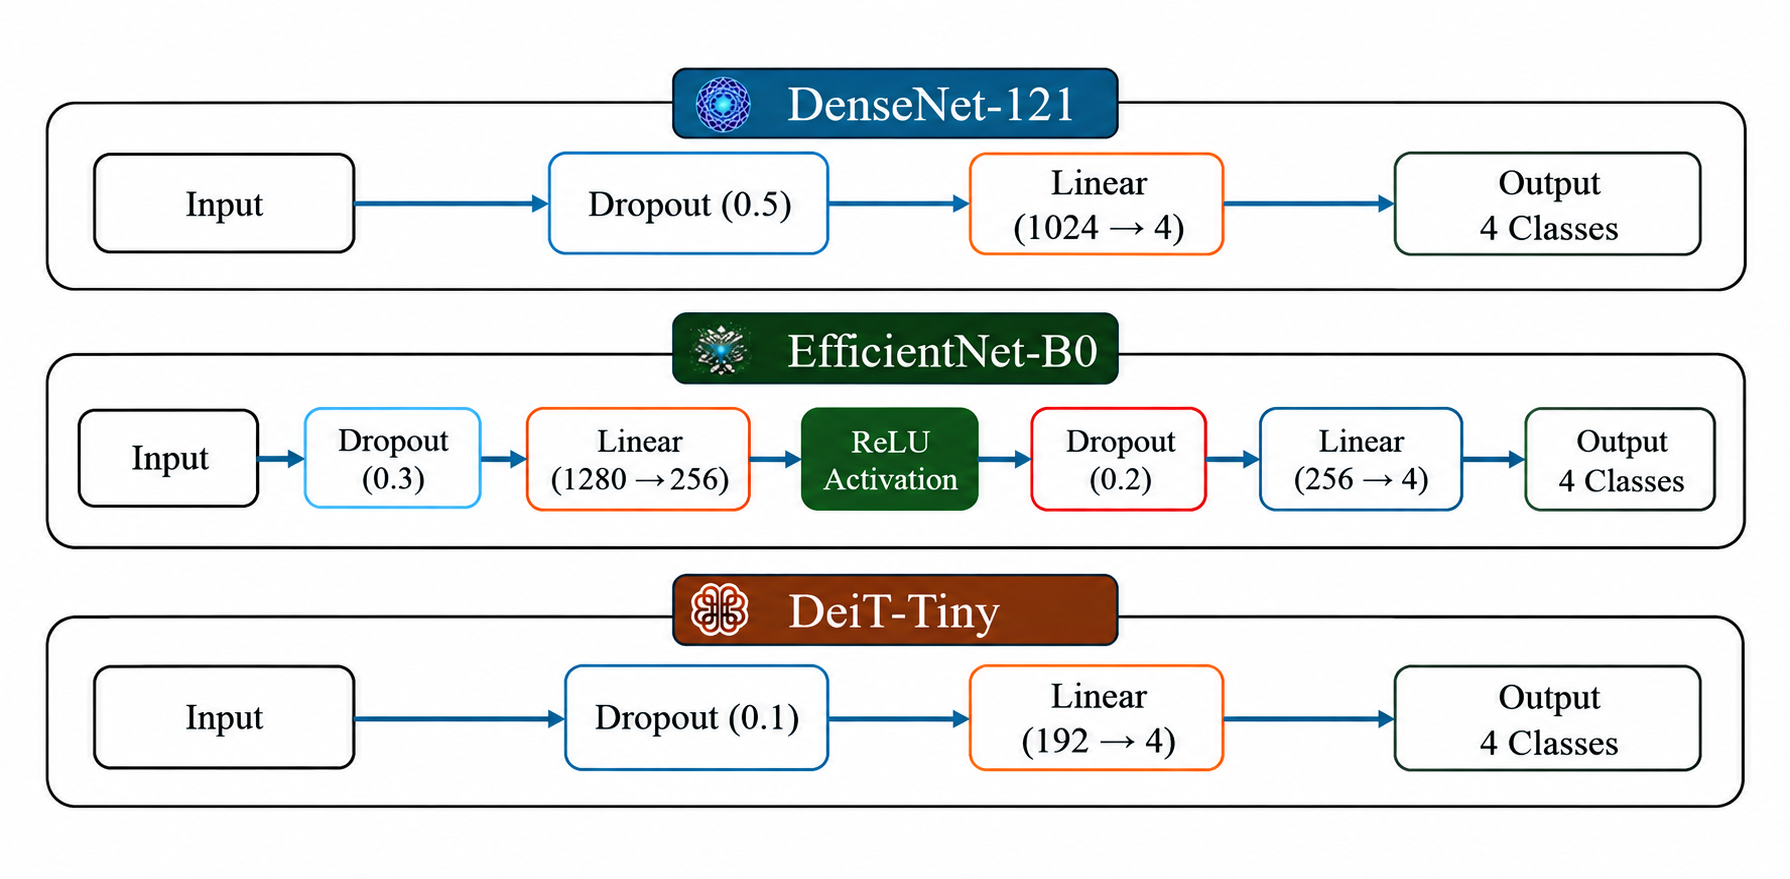
\includegraphics[width=\textwidth]{model_architectures_diagram.png}
  \caption{Task-specific classification head architecture appended to each
    pretrained backbone. DenseNet-121 and DeiT-Tiny use a single linear
    layer after dropout; EfficientNet-B0 uses a two-layer head with an
    intermediate ReLU activation}
  \label{fig:model_heads}
\end{figure}

Figure~\ref{fig:model_heads} illustrates the task-specific classification
head appended to each backbone. DenseNet-121~\citep{Huang2017} employs
dense connectivity in which each layer receives feature maps from all
preceding layers, promoting feature reuse.

EfficientNet-B0~\citep{Tan2019} applies compound scaling of depth,
width, and resolution jointly.

DeiT-Tiny~\citep{Touvron2021} processes $224\times224$ images as
196 non-overlapping $16\times16$ patch tokens through 12 self-attention
layers. Architecture-specific dropout rates were selected as regularization
hyperparameters, with rates of 0.5, 0.3, and 0.1 for DenseNet-121,
EfficientNet-B0, and DeiT-Tiny, respectively.

\subsection{Asymmetric Endoscopy Loss}
\label{sec:ael}

To provide a controllable mechanism for encoding the unequal clinical
implications of errors across risk tiers, we used a tunable risk-oriented
cost-sensitive weighted cross-entropy formulation, referred to as the
Asymmetric Endoscopy Loss (AEL). Mathematically, AEL is a weighted
cross-entropy objective with a fixed class-weight vector; it is not a new
mathematical family of loss functions. AEL is
intended as a tunable weighting scheme rather than a method guaranteed to
improve aggregate classification performance: the class weights allow the
relative penalty for High-Risk errors to be adjusted, trading overall
accuracy against safety-oriented recall for the highest-risk tier.

\begin{equation}
  \mathcal{L}_{\text{AEL}}(\mathbf{p}, y) =
    -\sum_{k=0}^{3} w_k\,\mathbf{1}[y=k]\,\log p_k, \quad
  \mathbf{w} = [1.0,\; 3.5,\; 3.0,\; 5.0]
  \label{eq:ael}
\end{equation}
where $\mathbf{p}$ denotes the softmax probability vector, $y$ is the
ground-truth class, and $w_k$ is the relative penalty assigned to class~$k$.

\subsubsection*{Clinical Cost Interpretation}

Let $\mathbf{C} \in \mathbb{R}_{\geq 0}^{4\times4}$ denote a conceptual
clinical cost matrix, where $C_{ij}$ represents the relative consequence
associated with predicting class~$j$ when the true class is~$i$
($C_{ii}=0$). Under a cost-sensitive decision framework, the expected cost
of assigning prediction $\hat{y}$ to an observation $\mathbf{x}$ can be
expressed as:
\begin{equation}
  \mathcal{R}(\hat{y} \mid \mathbf{x})
    = \sum_{i} P(y{=}i \mid \mathbf{x})
      \sum_{j} C_{ij}\,\mathbf{1}[\hat{y}{=}j].
  \label{eq:bayes_cost}
\end{equation}
In the present study, the cost matrix was not estimated from patient-level
outcomes. Instead, it was used as a conceptual framework for assigning
relative class weights that emphasize classes for which misclassification is
considered more consequential within the proposed risk-stratification
framework. The resulting weights are therefore treated as
relative training penalties rather than empirically estimated
clinical utilities. The High-Risk class received the largest weight
($w_3=5.0$) because errors involving this tier are of greatest concern
within the proposed safety-oriented classification framework.
The Inflammatory class received $w_1=3.5$, despite having fewer training
examples than the Pre-malignant class, while the Pre-malignant class
received $w_2=3.0$. Normal findings were assigned the baseline weight
$w_0=1.0$.

Accordingly, the weight vector should be interpreted as a
heuristic cost-sensitive weighting scheme informed by clinical risk
and class imbalance, rather than as a direct numerical estimate of
patient-level morbidity or mortality. Table~\ref{tab:ael_weights} summarizes
the rationale for each class weight.

\begin{table}[H]
\centering
\caption{AEL class weight rationale}
\label{tab:ael_weights}
\begin{tabular}{clr p{8.5cm}}
\toprule
\textbf{Class} & \textbf{Label} & \textbf{Weight} &
\textbf{Rationale within the proposed risk framework}\\
\midrule
0 & Normal        & 1.0 & Baseline reference category\\
1 & Inflammatory  & 3.5 & Greater penalty for errors involving inflammatory
                          findings and the relatively small class size\\
2 & Pre-malignant & 3.0 & Emphasizes errors involving findings requiring
                          further assessment or surveillance\\
3 & High-Risk     & 5.0 & Highest penalty because errors involving the
                          highest-risk tier are prioritized by the
                          safety-oriented objective\\
\bottomrule
\end{tabular}
\par\smallskip
{\footnotesize\textit{The weights are intended to guide model optimization
and do not represent validated clinical utilities, mortality ratios, or
treatment priorities. Actual clinical consequences depend on the individual
finding, patient context, diagnostic confirmation, and physician assessment.}}
\end{table}

\subsection{Training Protocol}
\label{sec:training}

All three architectures were trained using the same optimization and training
protocol to ensure a controlled comparison. Experiments were conducted on
Apple M2 hardware using the PyTorch MPS backend. The complete set of training
hyperparameters is provided in Table~\ref{tab:hparams}.

\begin{table}[H]
\centering
\caption{Training hyperparameters (identical for all three models)}
\label{tab:hparams}
\begin{tabular}{ll}
\toprule
\textbf{Hyperparameter} & \textbf{Value}\\
\midrule
Optimizer          & AdamW\\
Learning rate      & $2\times10^{-4}$\\
Weight decay       & $1\times10^{-4}$\\
LR schedule        & CosineAnnealingLR ($\eta_{\min}=1\times10^{-6}$)\\
Epochs             & 25\\
Batch size         & 32\\
Gradient clipping  & 1.0 (L$_2$ norm)\\
Class balancing    & WeightedRandomSampler\\
CLAHE clip limit   & 2.0\\
CLAHE tile grid    & $8\times8$\\
Random seed        & 42\\
\bottomrule
\end{tabular}
\end{table}

\begin{figure}[H]
  \centering
  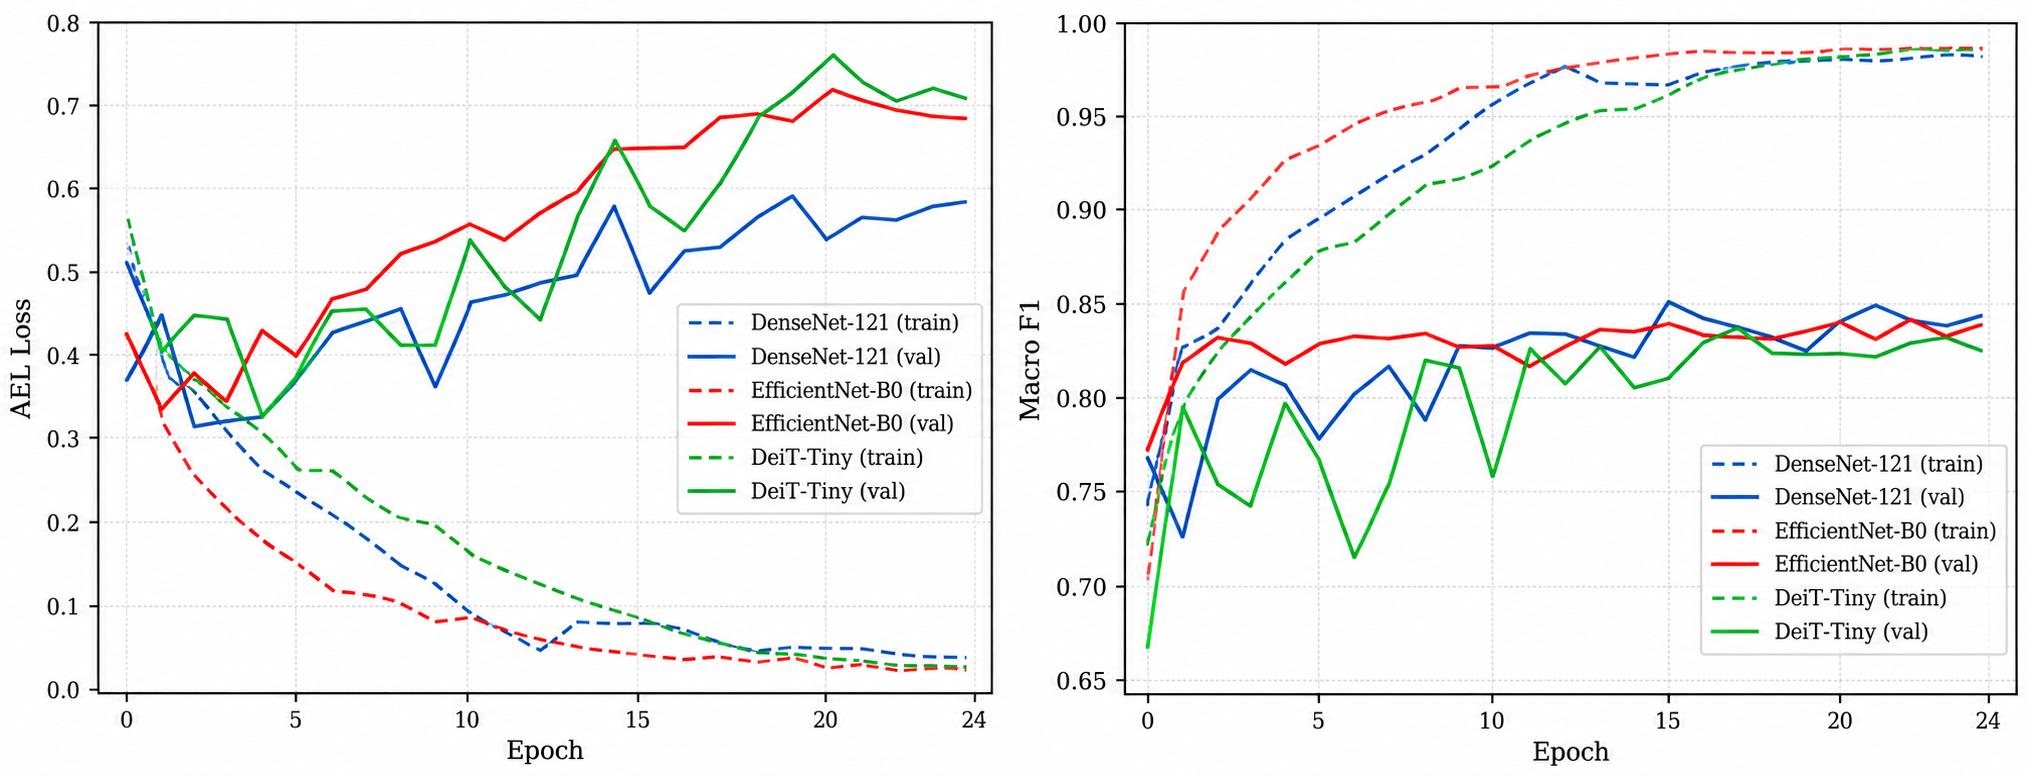
\includegraphics[width=\linewidth]{training_curves.png}
  \caption{Training and validation loss (left) and macro F1-score (right)
    over 25 epochs for DenseNet-121, EfficientNet-B0, and DeiT-Tiny.
    Solid lines show validation metrics; dashed lines show training metrics}
  \label{fig:training}
\end{figure}

Figure~\ref{fig:training} presents the training and validation loss and
macro F1-score over the 25 training epochs. Training loss decreased toward
near-zero values for all three architectures, while validation loss
increased after the early epochs and training macro F1 continued to improve
beyond the point at which validation macro F1 plateaued. Validation macro
F1 remained relatively stable despite the continued improvement in training
performance, suggesting some degree of train-validation divergence in later
epochs. This pattern indicates that longer training or stronger
regularization could be explored in future work.

\subsection{GradCAM Explainability}
\label{sec:gradcam}

GradCAM~\citep{Selvaraju2017} was used to visualize image regions
contributing to the predicted class. The method computes class-discriminative
localization maps by weighting convolutional feature channels according to the
average gradient of the target class score and applying a ReLU operation.

For DeiT-Tiny, which uses a token-based architecture rather than conventional
convolutional feature maps, the corresponding token-level gradients were
reshaped into a $14\times14$ spatial grid and subsequently upsampled to the
input-image resolution using bicubic interpolation.

\subsection{Monte Carlo Dropout Uncertainty Quantification}
\label{sec:mcdropout}

Monte Carlo (MC) Dropout~\citep{Gal2016} was used to estimate predictive
uncertainty by retaining dropout during inference and performing $T=30$
stochastic forward passes. The resulting predictions can be interpreted as
approximate samples from the model's posterior predictive distribution.

For an input image $\mathbf{x}$, predictive uncertainty was quantified as:

\begin{equation}
  U(\mathbf{x}) = 1 - \frac{1}{T}\sum_{t=1}^{T}\max_c\, p_c^{(t)}(\mathbf{x})
  \label{eq:uncertainty}
\end{equation}

where $p_c^{(t)}(\mathbf{x})$ is the predicted probability for class~$c$
during stochastic forward pass~$t$.

This measure, one minus the mean maximum softmax probability across
stochastic passes, was selected because it directly reflects the quantity
used by the referral rule itself: a confidence threshold applied to the
predicted class probability. Other uncertainty measures reported in the MC
Dropout literature, including predictive entropy, variation ratio, and
mutual information between predictions and model parameters, capture related
but distinct aspects of uncertainty (e.g., entropy reflects the full
predictive distribution rather than only the top class, and mutual
information attempts to isolate epistemic from aleatoric uncertainty). We
did not implement these alternative measures in the present study; a
comparison across uncertainty quantification methods, and their effect on
referral behavior, is a natural direction for future work.

For the workload-simulation experiment, an image was escalated for
endoscopist review when either of the following conditions was satisfied:
(i) predictive confidence was below the threshold $\tau=0.75$; or
(ii) the predicted class was Pre-malignant or High-Risk (class $\geq2$).

Thus, all predictions assigned to the two highest-risk categories were
automatically referred for review regardless of confidence. Under this
experimental referral rule, approximately 5\,\% of cases belonging to the
High-Risk category were predicted as Pre-malignant rather than High-Risk;
because both categories were escalated, these cases were included in the
referral set. No High-Risk ground-truth images in the internal test set were
predicted as either of the two lower-risk categories under the reported
experiment.

This result describes the behavior of the proposed classification-and-referral
protocol on the internal test set and should not be interpreted as evidence of
clinical sensitivity or the absence of missed lesions in clinical practice.

\subsection{Endoscopist Workload Simulation}
\label{sec:workload}

The proposed referral protocol was evaluated as a simulated
endoscopist-workload reduction strategy. Images with predictive confidence
$\geq\tau$ and predicted class $<2$ were considered eligible for automatic
clearance, whereas all other images were referred for endoscopist review.
The confidence threshold was evaluated over the range $\tau=0.60$ to $0.90$,
with the results at $\tau=0.75$ reported in Section~\ref{sec:results}.

Macro F1-score was used as the primary evaluation metric because of the class
imbalance across the four risk tiers. Secondary metrics included per-class
precision, recall, F1-score, and one-vs-rest AUC-ROC, all calculated on the
held-out internal test set.

\subsection{Five-Fold Cross-Validation and Confidence Intervals}
\label{sec:kfold}

The five-fold cross-validation described in this section is a separate,
independent robustness analysis and is distinct from the fixed 70\,\%/15\,\%/15\,\%
training/validation/test split used to obtain the primary results reported
in Section~\ref{sec:results} (Tables~\ref{tab:main_perf}
and~\ref{tab:per_class}, based on the single 1,145-image held-out test set).
To assess the robustness of model performance across alternative stratified
partitions, we additionally performed five-fold cross-validation on the
full 7,633-image HyperKvasir four-tier subset, independently of the 70/15/15
split. In each fold, approximately 80\,\% of the images were used for training and 20\,\%
for evaluation, with stratification performed by risk class.

For each fold and architecture, an independent training run was initialized
from the ImageNet-1K pretrained checkpoint and trained using the same
hyperparameters listed in Table~\ref{tab:hparams}. Fold-level
macro F1, macro AUC-ROC, and High-Risk recall were recorded and
summarized as mean\,$\pm$\,standard deviation across the five folds.

Ninety-five-percent confidence intervals were calculated using the Student's
$t$-distribution with four degrees of freedom:
\begin{equation}
  \text{CI}_{0.95} =
    \bar{\mu} \;\pm\; t_{0.975,\,4}\cdot\frac{s}{\sqrt{5}},
  \label{eq:ci}
\end{equation}
where $\bar{\mu}$ and $s$ denote the mean and sample standard deviation of
the five fold-level estimates.

\subsection{McNemar's Statistical Significance Test}
\label{sec:mcnemar_methods}

Pairwise differences in classification behavior between architectures were
evaluated using the continuity-corrected McNemar test~\citep{McNemar1947}
on the same held-out HyperKvasir test set ($n=1{,}145$). For a pair of
models $A$ and $B$, $b$ denotes the number of images correctly classified
by $A$ but incorrectly classified by $B$, while $c$ denotes the number
correctly classified by $B$ but incorrectly classified by $A$.

The continuity-corrected test statistic was calculated as:
\begin{equation}
  \chi^2 = \frac{(|b - c| - 1)^2}{b + c},
  \label{eq:mcnemar}
\end{equation}
which is approximately distributed as $\chi^2$ with one degree of freedom
under the null hypothesis of equal marginal error rates. Statistical
significance was evaluated at $\alpha=0.05$.

Because all architectures were evaluated on the same images, McNemar's
test provides a paired comparison of their binary correct/incorrect
predictions.

%% ============================================================================
\section{Results}
\label{sec:results}
%% ============================================================================

\subsection{Classification Performance}

Table~\ref{tab:main_perf} summarizes macro F1-score and per-class AUC-ROC
on the 1,145-image HyperKvasir internal test set using the same AEL
training configuration ($\mathbf{w}=[1.0,3.5,3.0,5.0]$). DenseNet-121
obtained a macro F1-score of 0.8419 and a mean AUC-ROC of 0.9730, while
DenseNet-121 and EfficientNet-B0 obtained the same High-Risk recall of 0.9659.

The observed macro F1-scores were 0.8419 for DenseNet-121, 0.8390 for
EfficientNet-B0, and 0.8106 for DeiT-Tiny. Pairwise McNemar tests found no
statistically significant difference between DenseNet-121 and EfficientNet-B0
($p=0.911$) or between DenseNet-121 and DeiT-Tiny ($p=0.080$). The comparison
between EfficientNet-B0 and DeiT-Tiny reached the prespecified significance
level ($p=0.034$). These results indicate that the observed differences in
overall prediction behavior should be interpreted together with the uncertainty
and cross-dataset results rather than solely from the point estimates of
macro F1.

\begin{table}[H]
\centering
\caption{Classification performance on HyperKvasir test set (AEL loss)}
\label{tab:main_perf}
\begin{tabular}{lccc}
\toprule
\textbf{Metric} & \textbf{DenseNet-121} & \textbf{EfficientNet-B0} &
\textbf{DeiT-Tiny}\\
\midrule
Macro F1-score          & \textbf{0.8419} & 0.8390        & 0.8106\\
High-Risk Recall        & \textbf{0.9659} & \textbf{0.9659} & 0.9505\\
AUC-ROC (Normal)        & 0.9913        & \textbf{0.9919} & 0.9914\\
AUC-ROC (Inflammatory)  & \textbf{0.9362} & 0.9234        & 0.9213\\
AUC-ROC (Pre-malignant) & 0.9675        & \textbf{0.9720} & 0.9623\\
AUC-ROC (High-Risk)     & 0.9972        & 0.9962        & \textbf{0.9986}\\
Mean AUC-ROC            & \textbf{0.9730} & 0.9709        & 0.9684\\
\bottomrule
\end{tabular}
\end{table}

Table~\ref{tab:per_class} presents the per-class precision, recall, and
F1-score for DenseNet-121. The High-Risk class achieved an F1-score of
approximately 0.98, whereas the Inflammatory class produced the lowest
F1-score (0.58). The latter is consistent with the substantially smaller
number of Inflammatory examples in the test set (97 images) and the greater
visual overlap that can occur among inflammatory and other mucosal findings.

\begin{table}[H]
\centering
\caption{Per-class performance for DenseNet-121, which achieved the highest macro F1-score on the internal test set, on HyperKvasir test set}
\label{tab:per_class}
\begin{tabular}{lcccc}
\toprule
\textbf{Class} & \textbf{Precision} & \textbf{Recall} & \textbf{F1-score}
& \textbf{Support}\\
\midrule
Normal (0)        & 0.96 & 0.94 & 0.95 & 450\\
Inflammatory (1)  & 0.58 & 0.58 & 0.58 &  97\\
Pre-malignant (2) & 0.84 & 0.89 & 0.86 & 275\\
High-Risk (3)     & 0.99 & 0.97 & \textbf{0.98} & 323\\
\midrule
Macro avg         & 0.84 & 0.84 & 0.84 & 1145\\
Weighted avg      & 0.91 & 0.90 & 0.91 & 1145\\
\bottomrule
\end{tabular}
\end{table}

\subsection{Cross-Dataset Generalization}

Table~\ref{tab:kv2_mapping} shows how the eight Kvasir-v2 classes were
mapped to the four-tier risk schema for zero-shot evaluation. Table~\ref{tab:xdataset}
then reports macro F1-score on the HyperKvasir internal
test set and the Kvasir-v2 external dataset using this mapping. All models were trained
exclusively on HyperKvasir and evaluated on Kvasir-v2 without fine-tuning,
adaptation, or additional training.

The resulting macro F1-scores on Kvasir-v2 were 0.7403 for DenseNet-121,
0.7749 for EfficientNet-B0, and 0.7644 for DeiT-Tiny. The corresponding
decreases relative to the internal HyperKvasir results were 0.1017, 0.0641,
and 0.0463, respectively. High-Risk recall remained above 0.97 for all three
architectures on Kvasir-v2.

These results demonstrate a measurable performance shift between the internal
and external datasets while showing that the models retained relatively high
recall for the High-Risk category under the proposed four-tier schema.

\begin{table}[H]
\centering
\caption{Kvasir-v2 class mapping to the four-tier risk schema for zero-shot evaluation.
  Classes with no severity grade (e.g.\ \texttt{esophagitis}) were conservatively
  assigned to the lowest applicable tier; the mapping was reviewed by co-author
  Mehjabin Ferdous against ACG/ESGE guidelines}
\label{tab:kv2_mapping}
\begin{tabular}{lp{7cm}c}
\toprule
\textbf{Kvasir-v2 Class} & \textbf{Rationale} & \textbf{Tier}\\
\midrule
normal-cecum & Normal anatomical landmark & 0 Normal\\
normal-pylorus & Normal anatomical landmark & 0 Normal\\
normal-z-line & Normal gastroesophageal junction & 0 Normal\\
esophagitis & Ungraded finding conservatively assigned to the inflammatory category & 1 Inflammatory\\
hemorrhoids & Consistent with the HyperKvasir mapping & 1 Inflammatory\\
polyps & Consistent with the HyperKvasir mapping & 2 Pre-malignant\\
dyed-lifted-polyps & Consistent with the HyperKvasir mapping & 3 High-Risk\\
dyed-resection-margins & Consistent with the HyperKvasir mapping & 3 High-Risk\\
\bottomrule
\end{tabular}
\end{table}

\begin{table}[H]
\centering
\caption{Cross-dataset generalization - macro F1 (train: HyperKvasir;
  evaluate: Kvasir-v2 zero-shot)}
\label{tab:xdataset}
\begin{tabular}{lcccc}
\toprule
\textbf{Model} & \textbf{HyperKvasir} &
\textbf{Kvasir-v2} & \textbf{F1 Drop} & \textbf{HR Recall (KV2)}\\
\midrule
DenseNet-121    & \textbf{0.8419} & 0.7403 & 0.1017 & 0.9715\\
EfficientNet-B0 & 0.8390 & \textbf{0.7749} & 0.0641 & 0.9945\\
DeiT-Tiny       & 0.8106 & 0.7644 & \textbf{0.0463} & \textbf{0.9960}\\
\bottomrule
\end{tabular}
\end{table}

\subsection{Five-Fold Cross-Validation Results}
\label{sec:kfold_results}

Table~\ref{tab:kfold} summarizes the five-fold cross-validation results.
DenseNet-121 produced a macro F1-score of $0.8485\pm0.0069$, macro AUC-ROC
of $0.9748\pm0.0037$, and High-Risk recall of $0.9582\pm0.0068$.
EfficientNet-B0 and DeiT-Tiny showed comparable performance across the
evaluated metrics, with the fold-level variation reported in
Table~\ref{tab:kfold}. The cross-validation results provide an additional
assessment of performance stability across different stratified partitions
of the HyperKvasir four-tier dataset.

\begin{table}[H]
\centering
\caption{5-fold cross-validation results on HyperKvasir (mean\,$\pm$\,std
  across 5 folds; 95\,\% CI in parentheses)}
\label{tab:kfold}
\resizebox{\textwidth}{!}{%
\begin{tabular}{lcccc}
\toprule
\textbf{Model} & \textbf{Macro F1} & \textbf{Macro AUC} & \textbf{HR Recall}\\
\midrule
DenseNet-121
  & $0.8485 \pm 0.0069$ & $0.9748 \pm 0.0037$ & $0.9582 \pm 0.0068$\\
  & (95\,\%\,CI: 0.840--0.857) & (95\,\%\,CI: 0.970--0.979) & (95\,\%\,CI: 0.950--0.967)\\
\addlinespace
EfficientNet-B0
  & $0.8361 \pm 0.0069$ & $0.9677 \pm 0.0045$ & $0.9517 \pm 0.0058$\\
  & (95\,\%\,CI: 0.828--0.845) & (95\,\%\,CI: 0.962--0.973) & (95\,\%\,CI: 0.944--0.959)\\
\addlinespace
DeiT-Tiny
  & $0.8250 \pm 0.0186$ & $0.9698 \pm 0.0039$ & $0.9549 \pm 0.0105$\\
  & (95\,\%\,CI: 0.802--0.848) & (95\,\%\,CI: 0.965--0.975) & (95\,\%\,CI: 0.942--0.968)\\
\bottomrule
\end{tabular}}
\par\smallskip
{\footnotesize 95\,\% CI via Student's $t$-distribution ($df=4$).}
\end{table}

\subsection{McNemar's Statistical Significance Test}
\label{sec:mcnemar_results}

Table~\ref{tab:mcnemar} presents the pairwise McNemar test results.
DenseNet-121 versus EfficientNet-B0 produced $p=0.911$, while DenseNet-121
versus DeiT-Tiny produced $p=0.080$. The EfficientNet-B0 versus DeiT-Tiny
comparison produced $p=0.034$ under the prespecified $\alpha=0.05$ threshold.

\begin{table}[H]
\centering
\caption{McNemar's test for pairwise model comparisons on HyperKvasir test set
  ($n=1{,}145$). $\chi^2$ statistic and $p$-value reported with continuity
  correction; $\alpha=0.05$}
\label{tab:mcnemar}
\begin{tabular}{llccl}
\toprule
\textbf{Model A} & \textbf{Model B} & $b$ & $c$ & $\chi^2$ ($p$)\\
\midrule
DenseNet-121    & EfficientNet-B0 & 39 & 41 & 0.013 ($p$\,=\,0.911)\\
DenseNet-121    & DeiT-Tiny       & 56 & 38 & 3.074 ($p$\,=\,0.080)\\
EfficientNet-B0 & DeiT-Tiny       & 50 & 30 & 4.513 ($p$\,=\,0.034)\\
\bottomrule
\end{tabular}
\par\smallskip
{\footnotesize $b$\,=\,cases correctly classified by Model A but not Model B;
  $c$\,=\,cases correctly classified by Model B but not Model A.
  Continuity-corrected McNemar's test; $\alpha=0.05$.}
\end{table}

\subsection{Comparison with Related Methods}

Tables~\ref{tab:sota_scope} and~\ref{tab:sota_capability} place the proposed
approach alongside representative GI endoscopy AI studies according to task
formulation, dataset, model scale, uncertainty quantification,
explainability, cross-validation, and clinical-guideline alignment. Because
the compared studies address different datasets, class definitions, and
prediction tasks, their numerical performance measures are not directly
comparable.

\begin{table}[H]
\centering
\caption{Comparison with representative GI endoscopy AI approaches
  (2016-2024): task scope and scale. $\dag$\,=\,binary task (different
  schema); direct macro F1 comparison across rows is not meaningful because
  class schemas and task definitions differ}
\label{tab:sota_scope}
\begin{tabular}{lp{3.2cm}p{2.6cm}cc}
\toprule
\textbf{Method} & \textbf{Task} & \textbf{Dataset} &
\textbf{Classes} & \textbf{Params}\\
\midrule
Tajbakhsh et~al.~\citep{Tajbakhsh2016}
  & Binary polyp detection$^\dag$
  & Colonoscopy video & 2 & -\\
Pogorelov et~al.~\citep{Pogorelov2017}
  & Multi-class GI classif.
  & Kvasir-v1 & 8 & -\\
Ebigbo et~al.~\citep{Ebigbo2019}
  & Gastric lesion eval.$^\dag$
  & Single-site EGD & 2 & $>$8\,M\\
Jha et~al.~\citep{Jha2020}
  & Polyp segmentation$^\dag$
  & Kvasir-SEG & - & $>$25\,M\\
Ahmad et~al.~\citep{Ahmad2021}
  & Survey/review
  & Multiple & - & -\\
\midrule
\textbf{Ours}
  & \textbf{4-class risk stratification}
  & \textbf{HyperKvasir+Kvasir-v2} & \textbf{4} & \textbf{$<$8\,M}\\
\bottomrule
\end{tabular}
\end{table}

\begin{table}[H]
\centering
\caption{Comparison with representative GI endoscopy AI approaches
  (2016-2024): methodological capabilities. UQ\,=\,uncertainty
  quantification; XAI\,=\,gradient-weighted explainability;
  CV\,=\,cross-validation}
\label{tab:sota_capability}
\begin{tabular}{lcccc}
\toprule
\textbf{Method} & \textbf{UQ} & \textbf{XAI} &
\textbf{CV} & \textbf{Clinical align.}\\
\midrule
Tajbakhsh et~al.~\citep{Tajbakhsh2016}  & No & No & No & No\\
Pogorelov et~al.~\citep{Pogorelov2017} & No & No & No & No\\
Ebigbo et~al.~\citep{Ebigbo2019}        & No & No & No & Partial\\
Jha et~al.~\citep{Jha2020}              & No & GradCAM & No & No\\
Ahmad et~al.~\citep{Ahmad2021}          & No & No & N/A & Partial\\
\midrule
\textbf{Ours} & \textbf{MC Dropout} & \textbf{GradCAM}
  & \textbf{5-fold} & \textbf{Informed by ACG/ESGE}\\
\bottomrule
\end{tabular}
\end{table}

The closest controlled comparison in the present study is the ablation
experiment in Table~\ref{tab:ablation}, in which DenseNet-121 was trained
using the same four-class schema without the proposed asymmetric weighting.
Under that controlled protocol, standard cross-entropy achieved a macro
F1-score of $0.8350\pm0.0058$.

The proposed framework combines three methodological components: (1) a
four-class risk schema informed by published clinical guidance, (2)
cost-sensitive training through the proposed AEL weighting scheme, and
(3) uncertainty-aware referral simulation using MC Dropout. These components
are evaluated separately through the classification, ablation, uncertainty,
and workload experiments.

Importantly, the proposed framework should be regarded as an
experimental clinical decision-support methodology, rather than a
validated clinical decision system.

\subsection{AEL Ablation Study}
\label{sec:ablation}

The ablation experiments were designed to isolate the effect of the loss
function. These experiments used random initialization and did not apply
CLAHE, thereby separating the loss-function comparison from the
pretrained-checkpoint and image-enhancement configuration used for the main
experiments. Consequently, the absolute macro F1-scores in
Table~\ref{tab:ablation} should not be directly compared with the main
results in Table~\ref{tab:main_perf}.

Each configuration was trained three times using independent random seeds
(42, 0, and 123). DenseNet-121 was evaluated under three loss functions:
(i) AEL with $\mathbf{w}=[1.0, 3.5, 3.0, 5.0]$, (ii) standard
cross-entropy with uniform class weights, and (iii) Focal Loss with
$\gamma=2$. All other training conditions, including optimizer, scheduler,
augmentation, and number of epochs, were held constant.

\begin{table}[H]
\centering
\caption{AEL ablation on DenseNet-121 (25-epoch runs, $N=3$ independent
  seeds; values show mean\,$\pm$\,std). Bold marks best mean per column.
  Controlled protocol: random initialization, no CLAHE - results are
  relative comparisons across loss functions, not directly comparable to
  Table~\ref{tab:main_perf} (pretrained-checkpoint protocol)}
\label{tab:ablation}
\begin{tabular}{lcc}
\toprule
\textbf{Loss function} & \textbf{Macro F1} & \textbf{High-Risk Recall}\\
\midrule
Cross-Entropy (uniform)              & $0.8350 \pm 0.0058$          & $0.9567 \pm 0.0051$\\
Focal Loss ($\gamma=2$)              & \textbf{$0.8361 \pm 0.0021$} & $0.9484 \pm 0.0039$\\
AEL $[1.0, 3.5, 3.0, 5.0]$ (Ours)  & $0.7821 \pm 0.0042$          & \textbf{$0.9587 \pm 0.0039$}\\
\bottomrule
\end{tabular}
\end{table}

Under this controlled ablation protocol, Focal Loss produced the highest mean
macro F1-score (0.8361), while the AEL configuration produced the highest
mean High-Risk recall (0.9587), at the cost of a lower macro F1-score
(0.7821) than either cross-entropy or Focal Loss.

Because only three independent seeds were used, these results should be
interpreted as a controlled sensitivity analysis rather than definitive
evidence of statistical superiority among the loss functions. In particular,
the ablation results do not demonstrate that AEL improves macro F1 over the
alternative losses under this protocol; rather, they illustrate the
trade-off AEL is designed to make, favoring High-Risk recall over overall
macro F1 at this weight configuration. This
outcome is consistent with the intended role of AEL as a tunable
risk-weighting mechanism rather than a method designed to outperform
standard baselines on aggregate metrics: its practical value lies in
allowing the High-Risk penalty to be adjusted in a controlled manner,
as examined directly in the weight-sensitivity analysis
that follows (Section~\ref{sec:ael_sensitivity}), rather than in improving
macro F1 for a fixed weight configuration.

\subsection{AEL High-Risk Weight Sensitivity}
\label{sec:ael_sensitivity}

To evaluate the sensitivity of performance to the chosen High-Risk penalty
($w_3 = 5.0$), we swept the High-Risk weight over $\{3.0, 4.0, 5.0, 6.0, 7.0\}$ while
fixing all other weights at $[1.0, 3.5, 3.0]$ and training DenseNet-121 for
25 epochs under otherwise identical conditions. Each configuration was run
three times with independent random seeds (42, 0, 123) to quantify
run-to-run variance; Table~\ref{tab:ael_sensitivity} reports mean\,$\pm$\,std
across seeds for macro F1 and High-Risk recall on the held-out test set.
Macro F1 peaks at $w_3 = 5.0$ (0.7821) and declines for higher penalties,
reflecting progressive specialization toward the High-Risk class at the
expense of global discrimination. High-Risk recall is highest at $w_3 = 6.0$
(0.9701); the non-monotone pattern across weights reflects run-to-run variance
at $N=3$ seeds, and gains beyond $w_3 = 5.0$ are within one standard deviation.
$w_3 = 5.0$ was therefore adopted as the operating point that achieves the
best macro F1 (0.7821) while maintaining competitive High-Risk recall (0.9587).
This sweep was restricted to a narrow range of High-Risk weights ($3.0$-$7.0$)
and to macro F1 and High-Risk recall as the only reported metrics. A more
complete characterization of the safety-performance trade-off that AEL
enables would extend this sweep to a wider range of weights (e.g., $1$-$10$)
and report additional operating-point metrics such as lower-risk false
negative rate and simulated referral rate at each setting, ideally
summarized in a single trade-off plot (High-Risk weight vs.\ macro F1 and
High-Risk recall). This more complete sensitivity analysis is left for
future work.

\begin{table}[H]
\centering
\caption{AEL High-Risk weight sensitivity (DenseNet-121, 25-epoch runs,
  $N=3$ independent seeds; values show mean\,$\pm$\,std).
  Base weights fixed at $[1.0, 3.5, 3.0, w_3]$; random initialization,
  no CLAHE - a controlled protocol to isolate the High-Risk weight
  effect independently of pretraining and augmentation.
  Bold marks the column-wise best; the adopted configuration ($w_3=5.0$)
  is highlighted in the row label. Values are from this controlled
  weight-sensitivity protocol and are not directly comparable with the
  pretrained-checkpoint main experiment reported in
  Table~\ref{tab:main_perf}}
\label{tab:ael_sensitivity}
\begin{tabular}{lcc}
\toprule
\textbf{AEL weights} & \textbf{Macro F1} & \textbf{High-Risk Recall}\\
\midrule
$[1.0, 3.5, 3.0, 3.0]$ & $0.7807 \pm 0.0047$ & $0.9525 \pm 0.0053$\\
$[1.0, 3.5, 3.0, 4.0]$ & $0.7803 \pm 0.0039$ & $0.9628 \pm 0.0000$\\
$\mathbf{[1.0, 3.5, 3.0, 5.0]}$ \textbf{(ours)} & \textbf{$0.7821 \pm 0.0042$} & $0.9587 \pm 0.0039$\\
$[1.0, 3.5, 3.0, 6.0]$ & $0.7761 \pm 0.0084$ & \textbf{$0.9701 \pm 0.0039$}\\
$[1.0, 3.5, 3.0, 7.0]$ & $0.7761 \pm 0.0023$ & $0.9690 \pm 0.0025$\\
\bottomrule
\end{tabular}
\end{table}

\subsection{Uncertainty Quantification and Workload Simulation}

Table~\ref{tab:workload} reports endoscopist workload simulation results for
DenseNet-121, which achieved the highest macro F1-score on the internal test
set, using MC Dropout ($T=30$ passes) with confidence threshold $\tau=0.75$.
Under the experimental referral rule,
43.1\,\% of cases were classified as eligible for automatic clearance, while
all Pre-malignant and High-Risk predictions were escalated for review. No
ground-truth High-Risk images appeared in the automatically cleared subset
on the evaluated test set.

\begin{table}[H]
\centering
\caption{Endoscopist workload simulation results (DenseNet-121, $\tau=0.75$, $T=30$ MC Dropout passes)}
\label{tab:workload}
\begin{tabular}{ll}
\toprule
\textbf{Metric} & \textbf{Value}\\
\midrule
Total test images          & 1,145\\
AI auto-cleared            & 494 (43.1\,\%)\\
Flagged for endoscopist    & 651 (56.9\,\%)\\
Simulated auto-clearance rate & 43.1\,\%\\
Missed High-Risk lesions (test set) & \textbf{0}\\
Confidence threshold $\tau$ & 0.75\\
MC Dropout passes $T$      & 30\\
\bottomrule
\end{tabular}
\end{table}

\begin{figure}[H]
  \centering
  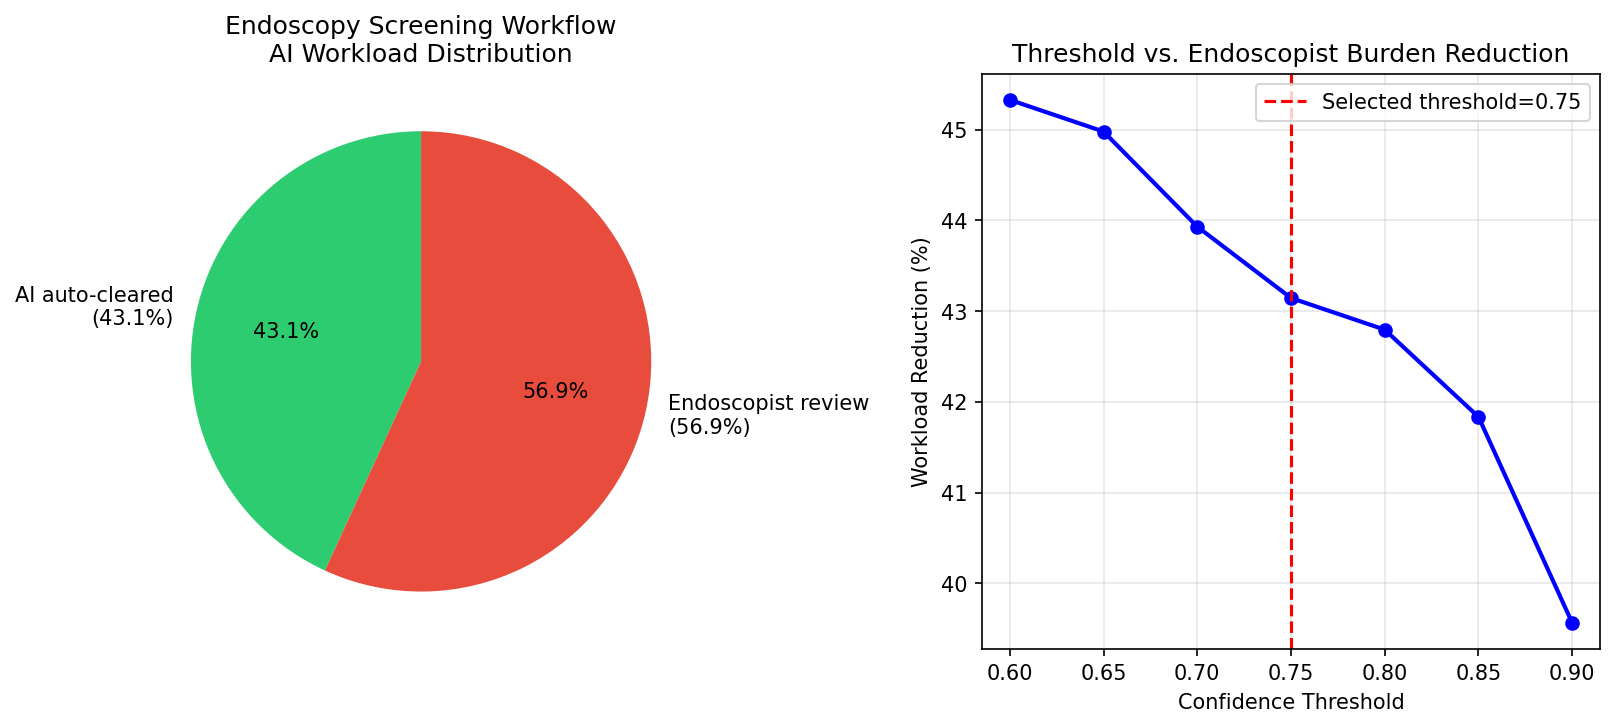
\includegraphics[width=\linewidth]{workload_simulation.png}
  \caption{Simulated auto-clearance rate (\%) and High-Risk escalation rate
    (\%) vs.\ MC Dropout threshold $\tau$ (DenseNet-121, $T=30$ passes).
    $\tau=0.75$ is marked; all High-Risk cases escalated regardless
    of confidence}
  \label{fig:workload}
\end{figure}

Figure~\ref{fig:workload} shows the simulated auto-clearance rate and
High-Risk escalation rate as a function of confidence threshold $\tau$,
swept from 0.60 to 0.90. Because auto-clearance requires predictive
confidence to meet or exceed $\tau$, higher confidence thresholds decrease
the simulated auto-clearance rate and correspondingly increase the number
of borderline cases referred for endoscopist review.
Because all Pre-malignant and High-Risk predictions are escalated regardless
of confidence, increasing $\tau$ affects only the clearance of Normal and
Inflammatory predictions. $\tau=0.75$ was selected as an intermediate
operating point balancing auto-clearance rate against the number of
borderline cases escalated. The threshold sweep
and evaluation were performed on the same held-out test split; in prospective
deployment, $\tau$ should be selected on an independent calibration cohort
and the workload-reduction estimate verified on a separate holdout.

\subsection{GradCAM Explainability}

\begin{figure}[H]
  \centering
  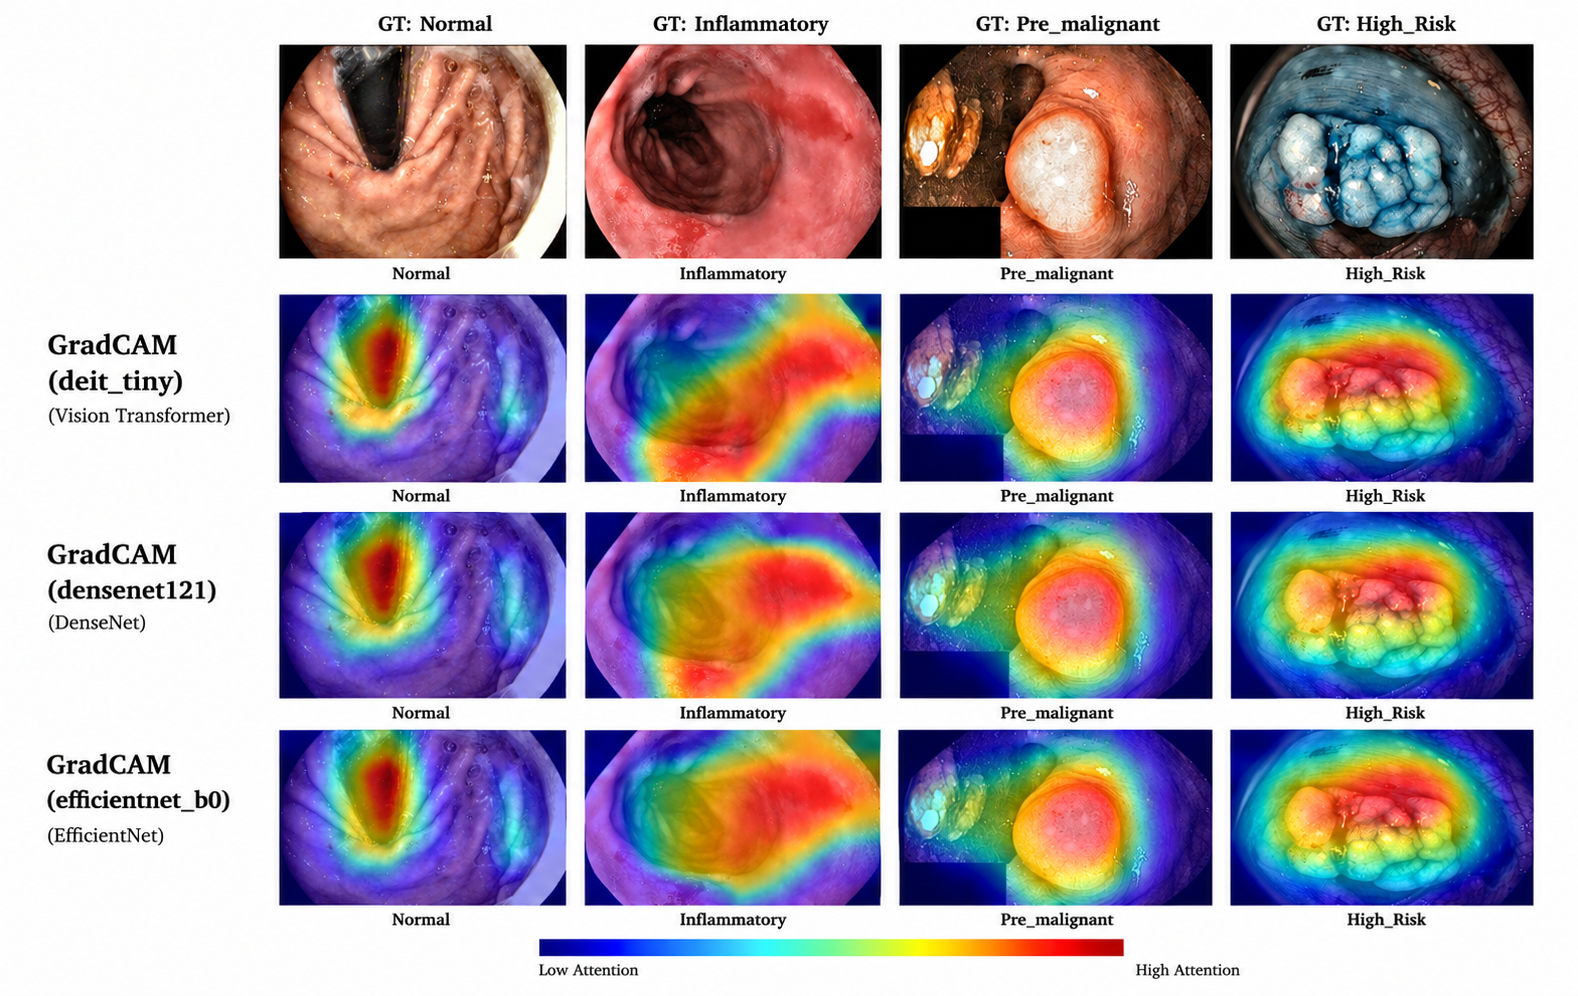
\includegraphics[width=\textwidth]{3models_gradcam.png}
  \caption{GradCAM heatmaps across four risk classes (Normal, Inflammatory,
    Pre-malignant, High-Risk) for all three architectures (DeiT-Tiny,
    DenseNet-121, EfficientNet-B0). Attended regions correspond qualitatively
    to visually relevant mucosal patterns. CNN architectures produce sharper,
    spatially localized attention; DeiT-Tiny shows broader patch-level
    patterns capturing global mucosal context}
  \label{fig:gradcam}
\end{figure}

Figure~\ref{fig:gradcam} shows representative GradCAM heatmaps for one image
per risk class across all three architectures. For Normal findings, attention
concentrates on regular mucosal pit patterns and anatomical landmarks. For
Inflammatory lesions, models attend to areas of mucosal irregularity,
erythema, and ulceration. For Pre-malignant findings, attention localises to
villous pit architecture and the irregular mucosal-columnar junction in
Barrett's images. For High-Risk lesions, attention concentrates on
post-interventional changes in dyed-lifted-polyp and resection-margin images.
CNN architectures produce sharper, more spatially localized heatmaps, while
DeiT-Tiny shows broader patch-level attention patterns capturing global
mucosal context. These observations describe qualitative localization
behavior only; GradCAM heatmaps cannot, on their own, establish that a
model relies on clinically valid diagnostic features.

\subsection{ROC Curves and Confusion Matrices}

\begin{figure}[H]
  \centering
  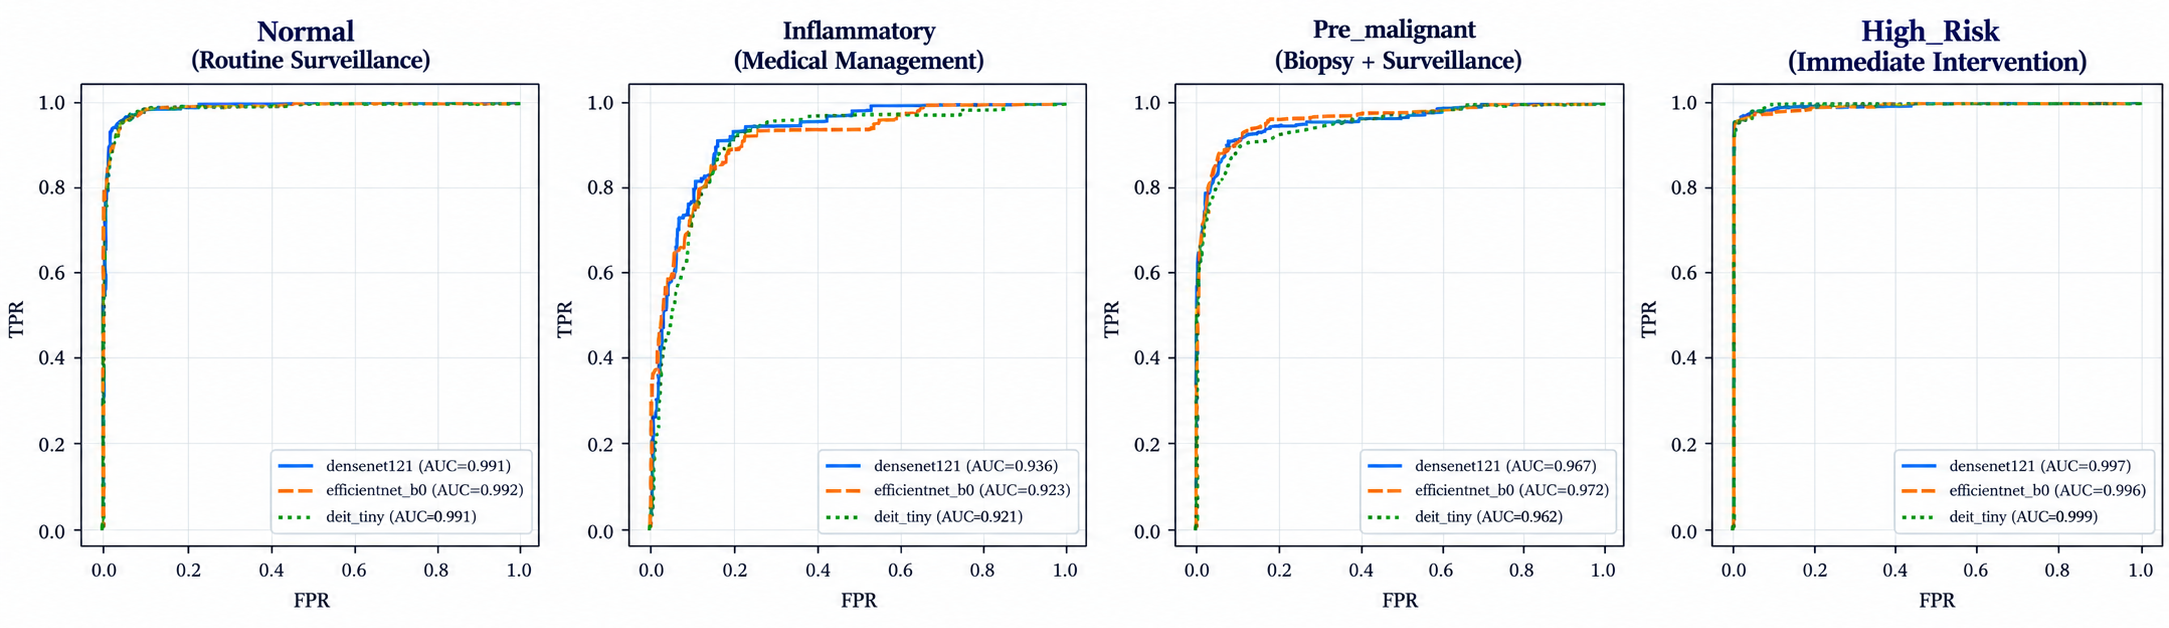
\includegraphics[width=\textwidth]{roc_curves.png}
  \caption{One-vs-rest ROC-AUC curves per risk class for all three models
    on the HyperKvasir test set}
  \label{fig:roc}
\end{figure}

Figure~\ref{fig:roc} presents one-vs-rest ROC curves for each risk class
on the HyperKvasir internal test set. All three architectures achieved high
mean AUC-ROC values, with DenseNet-121 obtaining 0.9730, EfficientNet-B0
0.9709, and DeiT-Tiny 0.9684. The High-Risk class produced the highest
AUC-ROC across the evaluated models, whereas the Inflammatory class
consistently produced the lowest AUC-ROC. The lower discrimination observed
for the Inflammatory category is consistent with the greater visual overlap
between inflammatory and normal mucosal appearances represented in the dataset.

\begin{figure}[H]
  \centering
  
\includegraphics[width=\textwidth]{confusion_matrix_combined.png}
  \caption{Normalized confusion matrices on the HyperKvasir test set for
    (a) DenseNet-121, (b) EfficientNet-B0, and (c) DeiT-Tiny. Rows represent
    true labels; columns represent predicted labels}
  \label{fig:cm}
\end{figure}

Figure~\ref{fig:cm} presents normalized confusion matrices for the three
architectures. The matrices show strong diagonal concentration across the
four risk categories. The most prominent error pattern occurs in the
Inflammatory class, where a proportion of cases are classified as Normal.
The Pre-malignant and High-Risk categories show comparatively strong
diagonal values across the evaluated architectures.

\subsection{Confusion Pattern Analysis}
\label{sec:confusion_analysis}

The confusion matrices reveal a consistent error pattern across the three
architectures. For DenseNet-121, Inflammatory recall was 0.58, indicating
that 58\,\% of the 97 Inflammatory test images were correctly identified.
The remaining errors were distributed primarily among neighboring risk
categories, with Normal being an important source of confusion.

The Pre-malignant class exhibited a precision of 0.84 and recall of 0.89,
indicating that the model identified most ground-truth Pre-malignant cases
while also assigning some lower-risk cases to this category. Within the
proposed referral protocol, predictions assigned to the Pre-malignant
category are escalated for specialist review; therefore, such errors increase
the referral burden rather than constituting automatic clearance.

DenseNet-121 achieved a High-Risk precision of 0.99 and recall of 0.97 on
the internal test set. The relatively high discrimination of this class may
partly reflect the distinctive visual characteristics of some HyperKvasir
classes assigned to the High-Risk tier, including dyed-lifted-polyps and
dyed-resection-margins.

Importantly, an Inflammatory-to-Normal error should not be interpreted as
clinically harmless. Although it does not represent a direct confusion
between the highest-risk categories, classification errors between adjacent
clinical categories may still have consequences because the proposed four-tier
schema is a simplified representation of clinical management. The present
dataset-level analysis cannot determine the clinical consequences of
individual misclassifications.

%% ============================================================================
\section{Discussion}
\label{sec:discussion}
%% ============================================================================

The experiments demonstrate that the proposed four-class image-classification
framework can achieve substantial discrimination across the defined risk
categories using models containing fewer than 8 million parameters. On the
HyperKvasir internal test set, DenseNet-121 achieved a macro F1-score of
0.8419 and mean AUC-ROC of 0.9730. EfficientNet-B0 achieved a macro F1-score
of 0.8390, while DeiT-Tiny achieved 0.8106.

Across the three architectures, High-Risk recall was at least 0.9505 on the
internal test set. Under the proposed referral simulation, predictions assigned
to either the Pre-malignant or High-Risk categories were automatically
escalated for review. Consequently, all ground-truth High-Risk cases in the
internal test set that were predicted as either class 2 or class 3 entered
the simulated referral pathway. This produced zero High-Risk cases among the
automatically cleared test images in the reported experiment.

This observation should be interpreted as a property of the
experimental referral rule and the evaluated test set, rather than as
a clinical safety guarantee. In particular, the rule cannot prevent a true
High-Risk lesion from being automatically cleared if the classifier
incorrectly predicts it as Normal or Inflammatory.

\subsection{CNN and Transformer Architectures}

The comparison of CNN- and Transformer-based architectures under the same
parameter-budget constraint provides an assessment of different
feature-learning approaches while limiting differences in model size.
DenseNet-121 and EfficientNet-B0 use convolutional feature extraction and
hierarchical local representations, whereas DeiT-Tiny uses patch tokens and
self-attention to model relationships across the image.

DenseNet-121 achieved the highest internal macro F1-score (0.8419), while
DeiT-Tiny achieved 0.8106. The difference was relatively modest in absolute
terms, and the corresponding McNemar comparison between DenseNet-121 and
DeiT-Tiny did not reach the prespecified significance level ($p=0.080$).
These results suggest that both local convolutional representations and
token-based global representations can capture discriminative information
in this four-class task.

The GradCAM visualizations provided qualitative evidence that model
activations were frequently concentrated around mucosal and lesion regions
rather than obvious image borders or textual overlays. However, qualitative
heatmaps cannot establish causal reliance on clinically meaningful features.
The broader activation patterns observed for DeiT-Tiny may reflect its
token-based representation and the spatial resolution of the reconstructed
attention map.

For High-Risk examples containing dyed-lifted-polyps or
dyed-resection-margins, the CNN-based models frequently produced localized
activations around visually prominent lesion or dye-boundary regions. These
observations are consistent with clinically interpretable image regions,
although further prospective evaluation would be required to determine whether
the highlighted regions reliably correspond to diagnostically relevant
structures.

\subsection{Cross-Dataset Generalization}

Performance decreased when models trained on HyperKvasir were evaluated on
Kvasir-v2 without fine-tuning. DenseNet-121 decreased from 0.8419 macro F1
on HyperKvasir to 0.7403 on Kvasir-v2, while EfficientNet-B0 decreased from
0.8390 to 0.7749 and DeiT-Tiny from 0.8106 to 0.7644.

The reduction in performance demonstrates the presence of a dataset-domain
shift despite the use of the same four-tier prediction schema. Differences in
image acquisition conditions, patient populations, endoscopic equipment,
illumination, and class composition may contribute to this shift. The present
experiments do not isolate the contribution of any individual factor.

Notably, the Normal-class recall for DenseNet-121 decreased substantially
between the internal and external datasets. This finding emphasizes that
strong internal performance does not necessarily translate directly to an
independent dataset.

From a healthcare informatics perspective, this cross-dataset evaluation is
one of the more informative aspects of the present study, because it tests
whether a model trained under one data-collection protocol retains useful
behavior when applied to images from a different patient population and
imaging system without any adaptation. This is a substantially more
demanding test of generalization than an internal held-out split from the
same dataset, and it is a common failure mode for clinical machine-learning
systems more broadly. The overall macro F1 drop (0.05-0.10 across
architectures) indicates that domain shift is a real and non-trivial effect
in this setting, consistent with prior reports of degraded performance for
GI endoscopy models evaluated outside their training distribution.
At the same time, High-Risk recall remained above 0.97 for all three
architectures on Kvasir-v2 despite the overall performance drop, suggesting
that whatever visual cues the models rely on for the High-Risk tier
transferred more robustly across datasets than the cues used for the other
tiers; however, this pattern should be interpreted cautiously given the
additional label-mapping uncertainty discussed in
Section~\ref{sec:limitations} and should not be read as evidence that the
system reliably generalizes as a whole.

Training and evaluating on multi-institutional datasets containing diverse
endoscopy systems would provide a more rigorous assessment of cross-site
robustness. Additional experiments using domain adaptation, color
normalization, or domain-generalization methods could also be investigated
in future work.

\subsection{Inflammatory Class Performance}

The Inflammatory category produced the lowest per-class F1-score for
DenseNet-121 (0.58). The relatively small representation of this category
in HyperKvasir (645 images compared with 1,836 Pre-malignant and 2,152
High-Risk images) limits the diversity of available training examples even
when class-balanced sampling is used.

In addition, some inflammatory findings may exhibit visual characteristics
that overlap with normal mucosa or neighboring risk categories. These factors
provide plausible explanations for the observed classification difficulty,
although the present study cannot distinguish their individual contributions.

The lower Inflammatory performance also demonstrates an important limitation
of the four-class formulation: clinically heterogeneous findings are grouped
into broad categories that may contain substantial visual and pathological
variation. Part of this difficulty may also reflect ambiguity in the
study-defined tier boundaries themselves rather than a purely visual
recognition problem: the Inflammatory tier sits directly between Normal and
Pre-malignant in the assumed risk hierarchy, and findings near either
boundary (e.g., mild esophagitis bordering on normal mucosa) may not have a
single unambiguous tier assignment. Rather than treating this weak class as
a result to obscure, we present it directly because it indicates where the
proposed risk schema is least reliable and therefore most in need of
refinement or expert re-examination in future work. Future work should
investigate finer-grained disease-specific classification and hierarchical
risk prediction.

\subsection{Clinical Workload Simulation}

The proposed referral protocol was evaluated as a simulation of potential
workload reduction rather than as a clinical workflow study. At the selected
confidence threshold of $\tau=0.75$, 43.1\,\% of the internal test images
were classified as eligible for automatic clearance under the experimental
rule.

The automatically cleared subset contained no ground-truth High-Risk images
in this particular test set. However, this observation should not be
interpreted as evidence that the system can safely replace endoscopist review.
The result depends on the prevalence, composition, and sampling
characteristics of the evaluated dataset.

Similarly, translating the simulated clearance percentage directly into saved
procedure time or additional clinical procedure slots would require prospective
workflow measurements. Review duration, case complexity, institutional
protocols, and the proportion of images per examination would all affect
actual workload.

Therefore, the reported 43.1\,\% value should be interpreted as an
experimental referral-rate estimate, not as a demonstrated clinical
workload reduction.

\subsection{Limitations}
\label{sec:limitations}

Several limitations should be considered.

First, HyperKvasir was collected at a single institution and therefore does
not capture the full variability of clinical endoscopy environments. Although
Kvasir-v2 provides an independent external evaluation dataset, it is not
equivalent to prospective multi-institutional validation.

Second, the four-class schema is a study-defined categorization rather than
an established clinical classification system, and it represents a
simplified representation of clinical risk (Section~\ref{sec:schema}).
Actual management depends on factors that may not be observable
from an endoscopic image alone, including lesion histology, morphology,
patient history, anatomical location, and physician assessment. Consequently,
the proposed classes should not be interpreted as direct clinical diagnoses
or treatment recommendations. Related to this, none of the risk tiers used in
this study, including Pre-malignant and High-Risk, are confirmed by
histopathological ground truth; assignments are based entirely on the
endoscopic finding labels provided with the source datasets. The terms
Pre-malignant and High-Risk should therefore be understood as
study-defined category labels rather than histologically validated
diagnoses. The present study also did not evaluate how sensitive the
reported results are to reasonable alternative class-to-tier mappings
(e.g., a more conservative assignment of \texttt{dyed-lifted-polyps} and
\texttt{dyed-resection-margins}, or an alternative placement of borderline
inflammatory findings). Quantifying this sensitivity, for example by
retraining under two or three alternative mappings and comparing the main
conclusions, would further strengthen confidence that the schema reflects a
genuine risk ordering rather than an arbitrary relabeling of HyperKvasir
classes, and is left for future work.

Third, the training, validation, and test partitions of HyperKvasir were
constructed at the image level (Section~\ref{sec:datasets}). HyperKvasir
does not provide patient or examination identifiers alongside its labelled
images, so it was not possible to explicitly verify or enforce that images
from the same patient or endoscopic examination were confined to a single
partition. If such images exist across partitions, this could lead to
optimistic performance estimates due to information leakage between
training and evaluation. This limitation should be considered when
interpreting the reported internal test-set performance.

Fourth, the mapping of Kvasir-v2 classes to the four-tier schema
(Table~\ref{tab:kv2_mapping}) was performed manually by the authors using
the same rationale applied to HyperKvasir. Because Kvasir-v2 uses a
different, coarser label taxonomy than HyperKvasir, this mapping introduces
an additional source of subjective judgment and potential label noise beyond
that already present in the study-defined HyperKvasir schema. The zero-shot
generalization results reported in Section~\ref{sec:results} should be
interpreted with this additional source of uncertainty in mind.

Fifth, the AEL weights were manually specified as a heuristic cost-sensitive
weighting scheme. They were not estimated from patient-level clinical outcomes
or a validated clinical utility function. The ablation experiment further
showed that AEL did not achieve the highest macro F1-score among the evaluated
loss functions. Therefore, the current experiments support the feasibility of
cost-sensitive training but do not establish that the selected weight vector
is optimal.

Sixth, MC Dropout with $T=30$ stochastic forward passes provides an
approximate uncertainty estimate rather than a direct measurement of clinical
uncertainty. This is particularly relevant because the referral protocol
(Section~\ref{sec:mcdropout}) relies on a fixed confidence threshold
($\tau=0.75$); if the underlying predicted probabilities are not
well-calibrated, this threshold does not correspond to a stable operating
point in terms of true error rate. The reported calibration results
indicate room for improvement in this respect. On the held-out test set,
the Expected Calibration Error (ECE) values were 0.069 for DenseNet-121,
0.074 for EfficientNet-B0, and 0.090 for DeiT-Tiny. Figure~\ref{fig:calibration}
presents the corresponding reliability diagrams, plotting observed accuracy
against predicted confidence for each model. All three models show
deviations from perfect calibration (the diagonal reference line) across
confidence bins, with no single consistent direction of bias across the
full confidence range. These values and patterns suggest that probability
calibration should be investigated further, for example via post-hoc
recalibration methods such as temperature scaling, before any clinical
application. The present study reports ECE and reliability diagrams but
does not report a proper scoring rule such as the Brier score; adding such
a metric, together with post-hoc recalibration, is left for future work.

\begin{figure}[H]
  \centering
  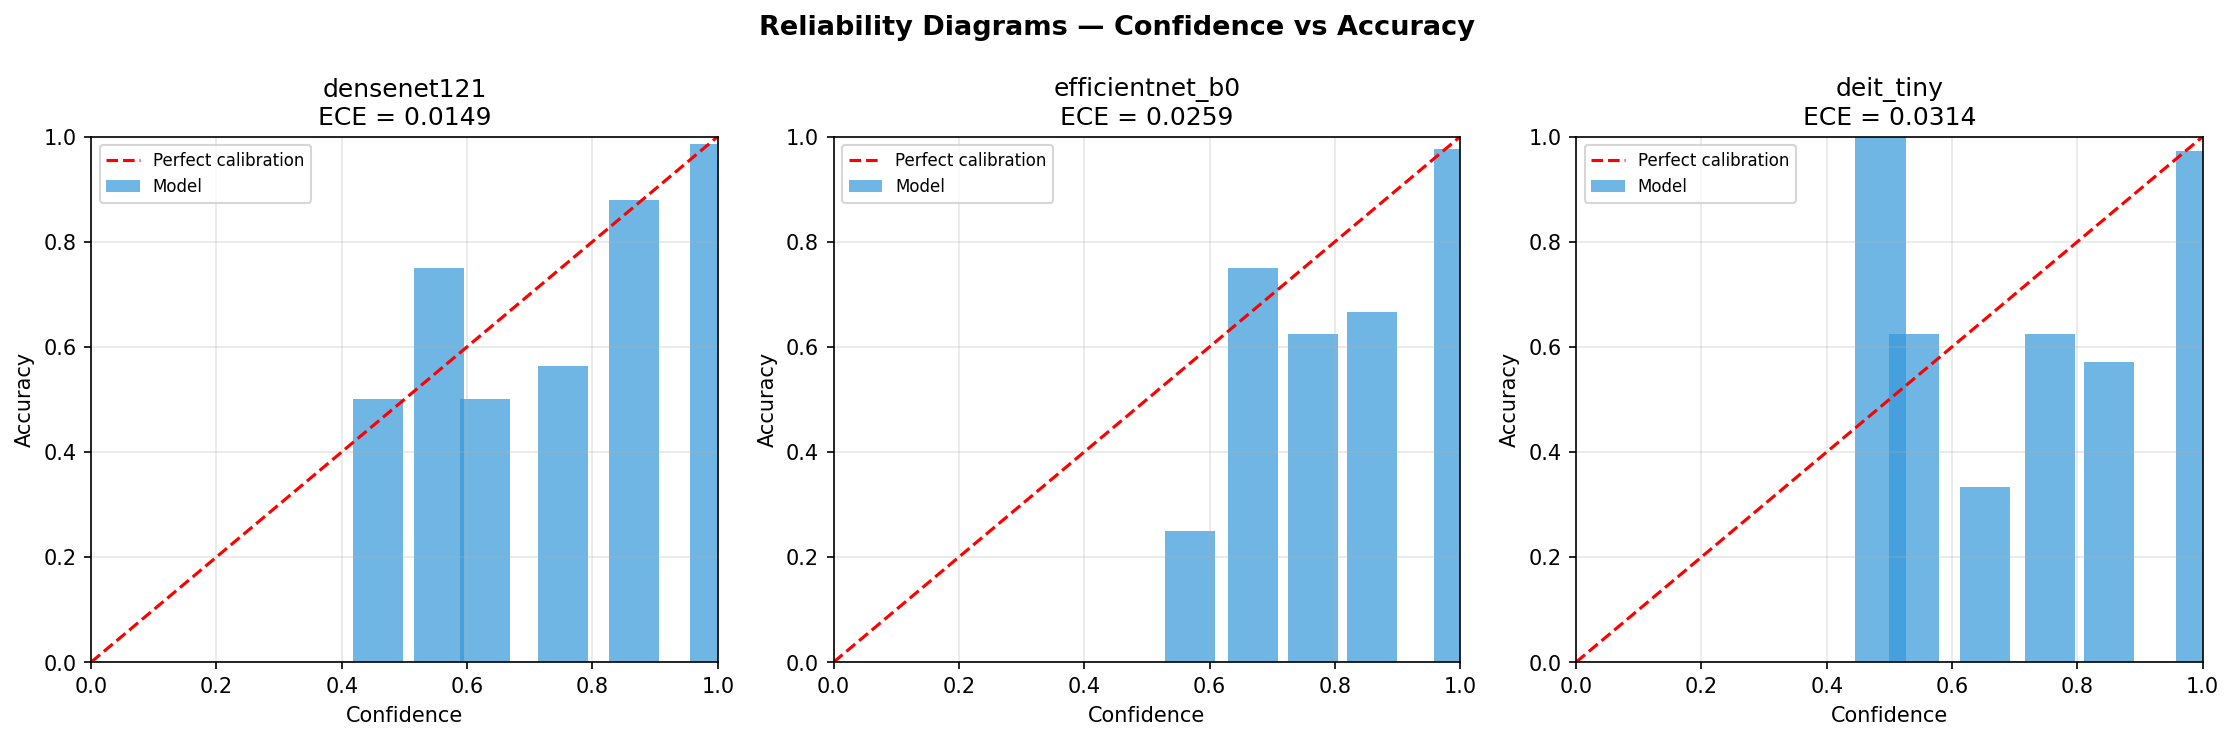
\includegraphics[width=\textwidth]{calibration_reliability.png}
  \caption{Reliability diagrams (confidence vs.\ observed accuracy) for
    DenseNet-121, EfficientNet-B0, and DeiT-Tiny on the HyperKvasir
    held-out test set. The dashed diagonal line represents perfect
    calibration; bars above the line indicate underconfidence in that bin,
    and bars below indicate overconfidence. Expected Calibration Error
    (ECE) is reported above each panel}
  \label{fig:calibration}
\end{figure}

Seventh, the five-fold cross-validation experiment was performed as a separate
robustness analysis on the full 7,633-image HyperKvasir subset. The resulting
estimates should not be interpreted as an independent external validation
because the same dataset was used for all folds.

Eighth, the McNemar analysis evaluates paired differences in binary
correct/incorrect predictions and does not establish clinical superiority of
one architecture. The significant EfficientNet-B0 versus DeiT-Tiny result
should therefore be interpreted specifically as evidence of a difference in
their paired error patterns on the evaluated test set.

Ninth, the endoscopist workload simulation (Section~\ref{sec:workload}) is a
retrospective, dataset-level simulation rather than a prospective clinical
evaluation. No clinicians interacted with the system in a live workflow, and
the simulated auto-clearance rate should not be interpreted as a measured
reduction in clinical workload.

Finally, all experiments were performed on Apple M2 MPS hardware. Parameter
count alone does not determine real-world inference latency because hardware
architecture, memory bandwidth, operator support, and quantization can
substantially affect runtime. DenseNet-121 achieved an average inference time
of approximately 14\,ms per image in the reported experimental environment,
but this measurement should not be generalized to clinical endoscopy hardware.
Dedicated benchmarking on representative deployment hardware would be necessary
before making real-time performance claims.

%% ============================================================================
\section{Conclusions}
\label{sec:conclusions}
%% ============================================================================

This study investigated a four-class GI endoscopy image-classification
framework that organizes findings into Normal, Inflammatory, Pre-malignant,
and High-Risk categories using a guideline-informed risk schema. Three
lightweight architectures (DenseNet-121, EfficientNet-B0, and DeiT-Tiny)
were evaluated using identical training conditions, external zero-shot
evaluation, five-fold cross-validation, GradCAM visualization, and MC
Dropout-based uncertainty estimation.

On the HyperKvasir internal test set, DenseNet-121 achieved a macro F1-score
of 0.8419 and mean AUC-ROC of 0.9730. EfficientNet-B0 achieved a macro
F1-score of 0.8390, while DeiT-Tiny achieved 0.8106. On the independent
Kvasir-v2 dataset, the corresponding macro F1-scores were 0.7403, 0.7749,
and 0.7644, demonstrating a measurable reduction in performance under dataset
shift.

The experiments also demonstrate the importance of evaluating models beyond
a single aggregate classification metric. Inflammatory findings remained
substantially more difficult to classify than the other risk categories,
while the High-Risk category achieved high recall on both the internal and
external evaluations. The proposed referral simulation further showed that
the rule-based escalation of Pre-malignant and High-Risk predictions can
reduce the proportion of cases eligible for automatic clearance under the
experimental conditions. However, this result represents a retrospective
dataset simulation and does not establish clinical safety or replacement of
specialist review.

The AEL formulation provides a tunable mechanism for incorporating asymmetric
risk considerations into model optimization, allowing the High-Risk penalty
to be adjusted rather than fixed by a single design choice. The controlled
ablation did not demonstrate superior macro F1 relative to standard baseline
loss functions at the selected weight configuration, and the observed
High-Risk recall advantage came at a substantial cost to overall macro F1;
accordingly, AEL's contribution should be understood as offering a
controllable trade-off between overall accuracy and
safety-oriented recall rather than a guaranteed improvement over simpler
alternatives on both metrics simultaneously. The selected weights should be regarded as an initial
heuristic rather than a validated clinical cost model.

Overall, the findings support further investigation of lightweight CNN and
Transformer architectures for multi-class GI endoscopy risk stratification.
The most important next step is prospective, multi-institutional validation
across diverse patient populations, endoscopy systems, and clinical workflows.
Future work should also investigate improved probability calibration,
finer-grained lesion classification, morphology-aware risk modeling, and
clinically validated cost functions before considering deployment in
real-world endoscopy practice.

%% ============================================================================
\noindent\textbf{Acknowledgements}\quad The authors received no specific
funding or institutional support beyond their affiliated institutions for
this work.

\section*{Statements and Declarations}

\noindent\textbf{Funding}\quad The authors received no specific funding
for this work.

\noindent\textbf{Competing Interests}\quad The authors declare no
competing interests.

\noindent\textbf{Author Contributions}\quad A.R.\ contributed the
conceptualization, methodology, software, formal analysis, investigation,
data curation, visualization, and wrote the original draft. N.U.A.\
contributed to software, validation, formal analysis, visualization, and
reviewed and edited the manuscript. K.R.C.\ contributed to
conceptualization, supervision, and reviewed and edited the manuscript.
M.F.\ contributed clinical guideline validation and resources, and
reviewed and edited the manuscript. J.S.J.N.\ contributed clinical
guideline validation and resources, and reviewed and edited the
manuscript. M.S.H.\ contributed to validation, data curation, and
reviewed and edited the manuscript. A.U.Z.\ contributed to supervision,
project administration, and reviewed and edited the manuscript.

\noindent\textbf{Data and Code Availability}\quad HyperKvasir~\citep{Borgli2020}
and Kvasir-v2~\citep{Pogorelov2017b} are publicly available datasets;
access details are provided in the original dataset publications. All
preprocessing steps (CLAHE parameters, resizing, augmentation), the
train/validation/test split procedure, the random seed ($42$), model
architectures, and training hyperparameters used to produce the reported
results are described in Section~\ref{sec:methods}
(Tables~\ref{tab:archs} and~\ref{tab:hparams}). Code and trained model
checkpoints will be released in a public repository upon acceptance.

\noindent\textbf{Ethics Approval and Consent to Participate}\quad This
study used only publicly available, fully anonymized datasets (HyperKvasir
and Kvasir-v2). No human subjects were recruited and no patient-identifiable
data were accessed. Institutional ethics approval was therefore not
required.

\noindent\textbf{AI-Assisted Writing Disclosure}\quad AI-assisted tools
were used solely for language and copy editing. All scientific content,
methodology, analysis, interpretation, and conclusions were developed and
verified by the authors.

%% ============================================================================

\begin{thebibliography}{99}

\bibitem{Sung2021}
Sung H, Ferlay J, Siegel RL et al (2021) Global cancer statistics 2020:
  {GLOBOCAN} estimates of incidence and mortality worldwide for 36 cancers
  in 185 countries. CA Cancer J Clin 71:209-249.
  https://doi.org/10.3322/caac.21660

\bibitem{Kaminski2017}
Kaminski MF, Thomas-Gibson S, Bugajski M et al (2017) Performance measures
  for lower gastrointestinal endoscopy: a {European Society of
  Gastrointestinal Endoscopy (ESGE)} quality improvement initiative.
  Endoscopy 49:378-397. https://doi.org/10.1055/s-0043-102186

\bibitem{Wang2019}
Wang P, Berzin TM, Glissen Brown JR et al (2019) Real-time automatic
  detection system increases colonoscopic polyp and adenoma detection
  rates: a prospective randomized controlled study. Gut 68:1813-1819.
  https://doi.org/10.1136/gutjnl-2019-318532

\bibitem{Ahmad2021}
Ahmad OF, Soares AS, Mazomenos E et al (2021) Artificial intelligence and
  computer-aided diagnosis in colonoscopy: current evidence and future
  directions. Lancet Gastroenterol Hepatol 6:849-861.
  https://doi.org/10.1016/S2468-1253(21)00099-X

\bibitem{Shaukat2021}
Shaukat A, Kahi CJ, Burke CA et al (2021) {ACG} clinical guidelines:
  colorectal cancer screening 2021. Am J Gastroenterol 116:458-479.
  https://doi.org/10.14309/ajg.0000000000001122

\bibitem{Ferlitsch2017}
Ferlitsch M, Moss A, Hassan C et al (2017) Colorectal polypectomy and
  endoscopic mucosal resection: {European Society of Gastrointestinal
  Endoscopy (ESGE)} clinical guideline. Endoscopy 49:270-297.
  https://doi.org/10.1055/s-0043-102569

\bibitem{Lin2017}
Lin TY, Goyal P, Girshick R et al (2017) Focal loss for dense object
  detection. In: Proceedings of the IEEE International Conference on
  Computer Vision (ICCV), Venice, pp 2980-2988.
  https://doi.org/10.1109/ICCV.2017.324

\bibitem{Tajbakhsh2016}
Tajbakhsh N, Gurudu SR, Liang J (2016) Automated polyp detection in
  colonoscopy videos using shape and context information. IEEE Trans Med
  Imaging 35:630-644.
  https://doi.org/10.1109/TMI.2015.2487997

\bibitem{Ebigbo2019}
Ebigbo A, Mendel R, Probst A et al (2019) Computer-aided diagnosis using
  deep learning for the evaluation of malignant potential of gastric
  subepithelial lesions. Sci Rep 9:4465.
  https://doi.org/10.1038/s41598-019-40997-8

\bibitem{Gal2016}
Gal Y, Ghahramani Z (2016) Dropout as a {Bayesian} approximation:
  representing model uncertainty in deep learning. In: Proceedings of the
  33rd International Conference on Machine Learning (ICML), New York,
  pp 1050-1059

\bibitem{Pogorelov2017}
Pogorelov K, Randel KR, Griwodz C et al (2017) {KVASIR}: a multi-class
  image dataset for computer aided gastrointestinal disease detection.
  In: Proceedings of the ACM Multimedia Systems Conference (MMSys),
  Taipei, pp 164-169. https://doi.org/10.1145/3083187.3083212

\bibitem{Borgli2020}
Borgli H, Thambawita V, Smedsrud PH et al (2020) {HyperKvasir}, a
  comprehensive multi-class image and video dataset for gastrointestinal
  endoscopy. Sci Data 7:283.
  https://doi.org/10.1038/s41597-020-00622-y

\bibitem{Jha2020}
Jha D, Smedsrud PH, Riegler MA et al (2020) Kvasir-SEG: a segmented
  polyp dataset. In: International Conference on Multimedia Modeling
  (MMM~2020). Lecture Notes Comput Sci 11962:451-462.
  https://doi.org/10.1007/978-3-030-37734-2\_37

\bibitem{Touvron2021}
Touvron H, Cord M, Douze M et al (2021) Training data-efficient image
  transformers and distillation through attention. In: Proceedings of the
  38th International Conference on Machine Learning (ICML), Virtual,
  pp 10347-10357

\bibitem{Dosovitskiy2021}
Dosovitskiy A, Beyer L, Kolesnikov A et al (2021) An image is worth
  $16\times16$ words: transformers for image recognition at scale.
  In: Proceedings of the International Conference on Learning
  Representations (ICLR), Vienna

\bibitem{Pogorelov2017b}
Pogorelov K, Randel KR, Espeland T et al (2017) Kvasir: a multi-class
  image dataset for computer aided gastrointestinal disease detection.
  In: Proceedings of the 8th ACM Multimedia Systems Conference (MMSys),
  Taipei

\bibitem{Reza2004}
Reza AM (2004) Realization of the contrast limited adaptive histogram
  equalization ({CLAHE}) for real-time image enhancement. J VLSI Signal
  Process 38:35-44.
  https://doi.org/10.1023/B:VLSI.0000028532.53893.82

\bibitem{Huang2017}
Huang G, Liu Z, van~der Maaten L, Weinberger KQ (2017) Densely connected
  convolutional networks. In: Proceedings of the IEEE Conference on
  Computer Vision and Pattern Recognition (CVPR), Honolulu,
  pp 4700-4708. https://doi.org/10.1109/CVPR.2017.243

\bibitem{Tan2019}
Tan M, Le QV (2019) {EfficientNet}: rethinking model scaling for
  convolutional neural networks. In: Proceedings of the 36th International
  Conference on Machine Learning (ICML), Long Beach, pp 6105-6114

\bibitem{Selvaraju2017}
Selvaraju RR, Cogswell M, Das A et al (2017) {Grad-CAM}: visual
  explanations from deep networks via gradient-based localization.
  In: Proceedings of the IEEE International Conference on Computer Vision
  (ICCV), Venice, pp 618-626.
  https://doi.org/10.1109/ICCV.2017.74

\bibitem{McNemar1947}
McNemar Q (1947) Note on the sampling error of the difference between
  correlated proportions or percentages. Psychometrika 12:153-157.
  https://doi.org/10.1007/BF02295996

\end{thebibliography}

%% ============================================================================
\section*{Authors and Affiliations}

\noindent
Azizur Rahman$^{1}$ \textperiodcentered\ Nakib Uddin Ahmed$^{2}$ \textperiodcentered\
Kadirur Rahman Chowdhury$^{3}$ \textperiodcentered\ Mehjabin Ferdous$^{4}$ \textperiodcentered\
J.S.\ Jannatun Nayema$^{5}$ \textperiodcentered\ Md.\ Shahadat Hossain$^{6}$ \textperiodcentered\
Akhlak Uz Zaman$^{7}$

\bigskip
\noindent
\Letter\ \textbf{Azizur Rahman} \\
\texttt{azizurusa22@gmail.com}

\noindent
\textbf{Nakib Uddin Ahmed} \\
\texttt{nakibuddin33@gmail.com}

\noindent
\textbf{Kadirur Rahman Chowdhury} \\
\texttt{kadirurrahmanchowdhury@gmail.com}

\noindent
\textbf{Mehjabin Ferdous} \\
\texttt{mehjabinferdousmu@gmail.com}

\noindent
\textbf{J.S.\ Jannatun Nayema} \\
\texttt{jsjannatunnayema23@gmail.com}

\noindent
\textbf{Md.\ Shahadat Hossain} \\
\texttt{shahadat.hossain.bio@gmail.com}

\noindent
\textbf{Akhlak Uz Zaman} \\
\texttt{akhlak@metrouni.edu.bd}

\bigskip
\noindent
$^{1}$ Department of Computer Technology (CAPS), Indiana Wesleyan University,
Marion, IN 46953, USA

\noindent
$^{2}$ Department of Information Technology, Shahjalal University of Science
and Technology, University Avenue, Sylhet-3114, Bangladesh

\noindent
$^{3}$ Birmingham City Business School, Faculty of Business, Law and Social
Sciences, Birmingham City University, Birmingham B4 7BD, UK

\noindent
$^{4}$ MPH, St.\ Francis College, 179 Livingston St, Brooklyn, NY 11201, USA

\noindent
$^{5}$ MPH, St.\ Francis College, 179 Livingston St, Brooklyn, NY 11201, USA

\noindent
$^{6}$ Department of Computer Science and Engineering, Metropolitan
University, Bateshwar, Sylhet-3104, Bangladesh

\noindent
$^{7}$ Department of Computer Science and Engineering, Metropolitan
University, Bateshwar, Sylhet-3104, Bangladesh

\end{document}
